\documentclass{classrep}
\usepackage[utf8]{inputenc}
\usepackage{color}
\usepackage{amsmath}
\usepackage{dirtytalk}
\usepackage{latexsym}
\usepackage{multirow}
\usepackage{graphicx}
\usepackage{float}
\newtheorem{exmp}{Przykład}[section]
\studycycle{Informatyka, studia STACJONARNE, I st.}
\coursesemester{VI}

\coursename{Komputerowe systemy rozpoznawania}
\courseyear{2020/2021}

\courseteacher{prof. dr hab. inż. Adam Niewiadomski}
\coursegroup{poniedziałek, 12:00}

\author{
  \studentinfo{Hubert Gawłowski}{224298} \and
  \studentinfo{Kamil Kiszko-Zgierski}{224328} }

\title{Projekt 1. Klasyfikacja dokumentów tekstowych}

\begin{document}
\maketitle

\section{Cel projektu}

Celem zadania jest zaimplementowanie algorytmu $k$-NN w technologii Java na potrzeby klasyfikacji tekstów
oraz zbadanie wpływu wybranych cech liczbowych i tekstowych na skuteczność powyższej metody. W wyniku działania algorytmu teksty zostaną przyporządkowane do krajów, z jakich pochodzą.
Badanie zostanie przeprowadzone na podstawie artykułów prasowych z agencji prasowej Reuters, które to pochodzą z 1987 roku, wszystkie teksty napisane są w języku angielskim, a przy klasyfikacji pod uwagę będą brane artykuły, które pochodzą z następujących krajów: Republika Federalna Niemiec, USA, Francja, Wielka Brytania, Kanada, Japonia.  \\


\section{Klasyfikacja nadzorowana metodą $k$-NN}
Algorytm $k$-NN (od angielskich słów nearest neighbour - najbliższy sąsiad) to algorytm, 
którego działanie polega na przyporządkowaniu obiektu poddanego rozpoznawaniu do jednej z klas.
 Do wykorzystania tego algorytmu niezbędny jest zestaw klas, do których może należeć obiekt, zbiór danych uczących oraz rozpoznawany obiekt.
Metoda $k$-NN należy do grupy metod minimalnoodległościowych, ponieważ o zaklasyfikowaniu obiektu 
do danej klasy decyduje najmniejsza odległość (zgodna z przyjętą metryką), pomiędzy rozpoznawanym obiektem oraz k-obiektami z ciągu uczącego. 
Wyszukiwanie najmniejszej odległości pomiędzy obiektami można przedstawić za pomocą wzoru ogólnego:
\begin{gather}
\rho(x, x ^ {i, k})= \min_{x^\mu \in U^i}(x, x^\mu)
\end{gather}
\indent gdzie $\rho$ to wybrana metryka, $U^i$ oznacza ciąg uczący, $x^{i, k}$ jest elementem zbioru $U^i$, a rozpoznawany obiekt to x \cite{tadeusiewicz90}.\\
\indent Skuteczność algorytmu $k$-NN  mierzona jest na podstawie odsetka poprawnych przyporządkowań obiektów do odpowiadających im klas. 


\subsection{Ekstrakcja cech, wektory cech}

Pierwszym etapem, który należy wykonać w procesie rozpoznawania tekstów jest wyodrębnienie takich cech, 
aby jak najlepiej określały ich charakterystykę.Wszystkie artykuły są napisane w tym samym języku oraz w tej samej formie stylistycznej, 
dlatego w trakcie analizy skupiliśmy się na cechach liczbowych oraz tekstowych. Mając to na uwadzę, dokonaliśmy ekstrakcji poniższych cech:
\begin{enumerate}
    \item Zapis cyfr - za pomocą analizy ciągu cyfr otrzymamy informacje o np. numerach telefonicznych, które to są charakterystyczne dla omawianego kraju. Z pomocą symboli matematycznych ceche tą możemy zapisać następująco:  
    \begin{equation}
        c_1 = \frac{|{s: s \in N \land s \in P_k}|}{w}
    \end{equation}
    gdzie $N$- zbiór ciągów cyfr znalezionych w dokumencie, $P$ - zbiór charakterystycznych ciągów cyfr dla danego kraju k (Słowniki charakterystycznych ciągów cyfr znajdują się w Załączniku 1), $w$ - waga przez jaką należy podzielić otrzymaną cechę.\\
    Wzór ten zastosujemy dla każdego z rozpatrywanych krajów i dzięki porównaniu otrzymanych wyników uzyskamy informacje do której grupy, na podstawie tej cechy, sklasyfikować dany dokument. \\
    \begin{exmp}Fragment artykułu pt. "Offers USA direct service in Denmark" \cite{reuters}\\
    \say{[...]The service allows callers in Denmark to reach an ATT
operator in the United States by dialing a single telephone
number, 0430-0010, ATT said.[...]}. \\
    \end{exmp}
Z powyższego fragmentu możemy wyodrębnić ciąg cyfr 0430-0010 i na jego podstawie sklasyfikować, do jakiej etykiety kraju możemy zaklasyfikować dany artykuł. Numery telefonów z różnych krajów mogą być rozpoznane na podstawie np. numeru kierunkowego, ich długości czy też formatu zapisu. \\
    \item Waluty - wyciągnięcie z tekstów nazw najczęsciej używanych walut. Każdy z krajów posługuje się inną walutą \footnote{Omawiane artykuły pochodzą z lat 80, kiedy we Francji i w Niemczech obowiązywała inna waluta (odpowiednio frank francuski i marka niemiecka). Kraje te przyjęły wspólną walutę, tj. euro dopiero w 2002 roku}, dlatego jest to cecha, która jasno charakteryzuje nam wybrane kraje. Wzory do tej cechy będą prezentowały się nasepująco:
	\begin{gather}
	    c_2' = d_{t}(M)
	\end{gather} 
    \indent gdzie $d_{t}$ jest funkcją wyznaczającą t najczęściej występujących słów w danym zbiorze, M to zbiór znalezionych w artykule słów oznaczających waluty. Zbiór walut charakterystycznych dla krajów znajduje się w Załączniku 1.
    \begin{gather}
        c_2 = g_k(c_2')
    \end{gather}
    \indent gdzie $g_k$ jest funkcją przyporządkowującą wyznaczone słowa do poszczególnego kraju k.\\
    W wyniku porównania otrzymanych dla każdego kraju wartości będziemy mogli stwierdzić do którego kraju, na podstawie tej cechy, można przyporządkować podany tekst.\\
    
    \begin{exmp}Fragment artykułu pt. "Maxtor agrees to acquire U.S. design" \cite{reuters}\\ 
    \say{[...]They said the arrangement, which is subject to a number of
    conditions including U.S. Design shareholder approval, calls
    for Maxtor to issue 12 mln dlrs worth of its own common stock
    in exchange for all of U.S. Design.[...]}. \\
    \end{exmp}
    W powyższym fragmencie została wymieniona waluta o nazwie dolar ("dlrs"). Mimo, że najbardziej popularnym dolarem jest dolar amerykański, natomiast na świecie jest jeszcze wiele innych walut, których pierwszym członem jest słowo "dolar", np. dolar kanadyjski, dolar australijski. Ten fakt należy również wziąć pod uwagę w momencie wyznaczania zbiorów rozmytych. Z podanego fragmentu wynika także, że aby w pełni skorzystać z tej cechy, należy uwzględnić nie tylko pełne nazwy walut, ale również ich skróty, które również się pojawiają w artykułach. \\
    \item Częstość występowania dat - zliczenie, jak często w podanych tekstach występują elementy określające czas. Wydaje się, że ich częstość będzie się różnić w zależności od pochodzenia tekstu. Powyższą cechę można przedstawić następująco:
    \begin{equation}
        c_3 = \frac{|{s: s \in D \land s \in A}|}{|A|}
    \end{equation}
    gdzie $D$ - zbiór słów oznaczających daty (zbiór formatów dat, według których słowo będzie klasyfikowane jako data znajduje się w Załączniku 1), $A$ - zbiór wszystkich słów z artykułu. \\
    \begin{exmp} Fragment artykułu pt. "USDA comments on export sales"  \cite{reuters} \\
    \say{[...]  In comments on its Export Sales Report, the department said
    sales of 1.0 mln tonnes to the USSR -- previously reported
    under the daily reporting system -- were the first sales for
    delivery to the USSR under the fourth year of the U.S.-USSR
    Grains Supply Agreement, which began October 1.
    [...]
        Egypt, Japan and Iraq were the major wheat buyers for
    delivery in the current year, while sales to China decreased by
    30,000 tonnes for the current season, but increased by 90,000
    tonnes for the 1987/88 season, which begins June 1. [...]}. \\
    \end{exmp}W przytoczonym fragmencie zapis daty został wykorzystany 3 razy ("October 1", "1987/88", "June 1"). Wobec tego, uważamy, że opisywana cecha będzie korzystnie wpływać na proces klasyfikacji tekstów. \\

    \item Format zapisu dat - w zależności od kraju format zapisu dat różni się. Cechę tą zapisać można za pomocą wzorów:
    \begin{gather}
        c_4' = f(B)
    \end{gather}
    \indent gdzie f - funkcja wyznaczająca zapis datowy z podanego zbioru, B - zbiór wszystkich wyrażeń znajdujących się w artykule (wyrażenie traktujemy jako połączenie minimum dwóch słów). Formaty zapisu dat, jakie będą brane pod uwagę przy wyznaczaniu znajdują się w Załączniku 1.
    \begin{gather}
        c_4 = t_k(c_4')
    \end{gather}
    \indent gdzie $t_k$ jest funkcją przyporządkowującą wyznaczone wyrażenia do poszczególnego kraju k.\\
    Jako, że w kilku krajach stosowany jest ten sam zapis datowy, funkcja ta może (a wręcz jest to bardzo prawdopodobne) zwrócić taką samą wartość dla kilku krajów. W wyniku porównania otrzymanych dla każdego kraju wartości będziemy mogli stwierdzić do którego kraju (bądź kilku krajów z równym prawdopodobiństwem), na podstawie tej cechy, można przyporządkować podany tekst. 
    \\
    
    \begin{exmp} Fragment artykułu pt. "Software services extends warrants" \cite{reuters} \\ \say{[...]Software Services of America
    Inc said its board has extended the expiration date of its
    warrants until August 31 from April 30.[...]}\\
    \end{exmp} Daty występujące w tym fragmencie ("August 31" i "April 30") są zapisane w formacie: miesiąc dzień. Uważamy, że w zależności od tego, z jakiego kraju pochodzi artykuł format zapisu dat może się różnić. \\
    \item Ogólna liczba słów - zliczenie wszystkich słów występujących w tekście. Uważamy, że w zależności od tego, jakiego kraju tekst dotyczy, ich długość może być różna. Liczbę wyrazów znajdujących się w tekście można przedstawić następująco:
    \begin{equation}
        c_5 = |A|
    \end{equation}
    gdzie $A$ - zbiór wszystkich słów z artykułu. \\
    \item Częstość słów rozpoczynających się wielką literą - słowa takie będą oznaczały najczęściej  nazwy własne np. imiona, nazwiska, nazwy budynków lub będą to rozwinięcia skrótów. Pisząc o jednym kraju może być używane więcej takich słów, 
	a o innych mniej. Z tej grupy wykluczymy jednak wyrazy składające się wyłącznie z wielkich liter (o których mowa będzie w punkcie następnym) oraz słowa pisane z wielkiej litery z uwagi na początek zdania. Aby odróżnić wielkie litery od małych, trzeba na początku dokonać odwzorowania liter w słowie na kody ASCII i następnie sprawdzić, czy odpowiedni kod ASCII znajduje się w przedziale od 65 do 90. W postaci wzoru wygląda to następująco:
	\begin{equation}
	f(l) = \begin{cases} 1 &\mbox{ jeśli }  l\in<65,90> \\ 0 & \mbox{ jeśli } l\notin<65,90> \end{cases}
	\end{equation}
	gdzie l oznacza pojedyńczy znak zapisany za pomocą kodu ASCII, a funkcja f(l) zwraca 1 dla liter zapisanych wielką literą, a 0 dla pozostałych znaków.
	Natomiast w celu obliczenia częstości słów rozpoczynających się wielką literą należy skorzystać z poniższego wzoru: 
	\begin{equation}
        c_6 = \frac{|{s: s \in Z \land s \notin W \land s \notin M}|}{|A|}
    \end{equation}
    gdzie $Z$ - zbiór słów, rozpoczynających się w arrtykule wielką literą, $A$ - zbiór wszystkich słów z artykułu, $W$ - zbiór słów, pisanych w artykule wielkimi literami, $M$ - zbiór słów, które rozpoczynają w artykule zdania. \\
	\begin{exmp}Fragment artykułu pt. "U.S. Auto Union will fight to stop job/wage cuts" \cite{reuters}\\
	\say{[...]The United Auto Workers union (UAW)
    vowed to fight wage and job cuts in a round of labour talks
    starting in July that cover nearly 500,000 workers at General
    Motors Corp and Ford Motor Co[...]}. \\
    \end{exmp}
    W tym krótkim fragmencie występuje aż 9 słów rozpoczynających się wielką literą, jednocześnie nie będących pierwszym słowem w zdaniu oraz nie będących słowem składających się tylko z wielkich liter. Słowa te są w tym fragmencie związane z nazwami własnymi oraz nazwą miesiąca. Uważamy, że przede wszystkim stosowanie nazw własnych może być związane z tym, z jakiego kraju pochodzi podany dokument. \\
    \item Częstość słów pisanych wielkymi literami - najczęściej będą to skróty. Uważamy, że w zależności od opisywanego kraju, ilość wykorzystywanych skrótów może się różnić. Do policzenia wystąpień słów zapisanych wielkimi literami należy wykorzystać poniższy wzór:
    \begin{equation}
        c_7 = \frac{|{s: s \in W}|}{|A|}
    \end{equation}
    gdzie $W$ - zbiór słów, pisanych w artykule wielkimi literami, $A$ - zbiór wszystkich słów z artykułu. \\ 
    \begin{exmp}Fragment artykułu pt."France approves large defence spending increase" \cite{reuters} \\
    \say {[...]The budget represents a six pct annual increase, starting next year, well above the 3.5 pct NATO recommends for members of its military command. France is a member of NATO but does
    not belong to its integrated military command.[...]} \\
    \end{exmp}
    W powyższym fragmencie skrót NATO(Organizacja Traktatu Północnoatlantyckiego) występuje 2 razy. Według nas, częstość występowania skrótów, w danym artykule może mieć związek z tym, jakiego kraju dotyczy tekst. \\
    \item Układ SI/imperialny - zdecydowanie częściej w artykułach z krajów anglojęzycznych będzie stosowany układ imperialny, natomiast w pozostałych - układ SI. 
    Wyliczenie liczby wystąpień jednostek w układzie SI można wyrazić następująco: 
     \begin{equation}
        c_8' = \frac{|{s: s \in S \land s \in A}|}{|A|}
    \end{equation}
    gdzie $S$ - zbiór słów oznaczających jednostki układu SI, $A$ - zbiór wszystkich słów z artykułu. \\
    Z kolei wzór do wyliczenia liczby wystąpień jednostek w układzie imperialnym przedstawia się w poniższy sposób:
    \begin{equation}
        c_8'' = \frac{|{s: s \in I \land s \in A}|}{|A|}
    \end{equation}
    gdzie $I$ - zbiór słów oznaczających jednostki układu imperialnego, $A$ - zbiór wszystkich słów z artykułu.\\ Zbiór słów oznaczających jednostki układu SI oraz układu imperialnego znajduje się w Załączniku 1.\\
    Jako opisywaną cechę zapisujemy różnicę wystąpień jednostek w układzie SI oraz imperialnym, czyli:
    \begin{equation}
        c_8 = {c_8'}-{c_8''}
    \end{equation} \\
    \begin{exmp}Fragment artykułu pt. "Sun in North Dakota oil find" \cite{reuters} \\
    \say{[...]flowed 660 barrels of oil and 581,000 cubic feet of natural gas per day through a 13/64 inch choke from depths of 13,188 to 13,204 feet.[...]}. \\
    \end{exmp}
    W powyższym tekście można zauważyć występowanie jednostkek z układu imperialnego, tj. cale(inch) i stopy(feet). Wobec tego, można przypuszczać, że tekst ten pochodzi z jednego z krajów anglojęzycznych. \\
    \item Częstość występowania cytatów - 
     kolejna cecha, która wydaje się różnić w zależności od kraju, o którym mowa w artykule. Liczba cytatów zostanie uzyskana w wyniku obliczenia liczby występowania słów, gdzie przedostatni znak to ',' lub '.', a ostatni '"'. Wyznaczenie  tej  cechy  można zaprezentować w postaci wzoru:
    \begin{equation}
        c_9 = \frac{|{s: s \in Y}|}{|A|}
    \end{equation}
    gdzie $Y$ - zbiór cytatów występujących w artykule, $A$ - zbiór wszystkich słów z artykułu. \\
    \begin{exmp}Fragment artykułu pt. "Hughes changes stance on merger after suit" \cite{reuters} \\
    \say{[...]"I think the merger is not going through," said Phil Pace,
    analyst at Kidder, Peabody and Co. He said the merger "lost a
    lot of its appeal" when the U.S. Department of Justice required
    that Baker sell off its Reed Tool Co operation.[...]}. \\
    \end{exmp}
    W podanym fragmencie cytat wystąpił 2 razy. Uważamy, że artykuły dotyczące różnych krajów będą też zawierały różną liczbę cytatów. \\

    \item Słowa kluczowe - sporządzone zostaną listy elementów identyfikujących każdy z krajów. Określenia te będą związane z elementami charakterystycznymi dla danego kraju. Możemy do nich zaliczyć nazwy geograficzne, znane osoby, nazwy firm itp.. Do wyznaczenia słów kluczowych należy skorzystać ze wzoru: 
    \begin{equation}
        c_{10} = \frac{|{s: s \in K \land s \in A}|}{|A|}
    \end{equation}
    gdzie $K$ - zbiór słów kluczowych (zbiory słów kluczowych dla każdego kraju znajdują się w Załączniku 1), $A$ - zbiór wszystkich słów z artykułu. \\
    \begin{exmp}Fragment artykułu pt. "Currency futures to key off G-5, G-7 meetings" \cite{reuters} \\
    \say{[...]News of an agreement among G-5 and G-7
    finance ministers meeting in Washington this week will be key
    to the direction of currency futures at the International
    Monetary Market, but any such agreement will need to go beyond
    the Paris accord to stem the recent rise in futures, financial
    analysts said.[...]}. \\
    \end{exmp}
    Powyższy tekst zawiera 2 słowa kluczowe - Washington i Paris. Washington związane jest z USA, natomiast Paris z Francją. Chcąc przyporządkować ten fragment biorąc pod uwagę tylko i wyłącznie cechę związaną ze słowami kluczowymi zostałby dopasowany z równym prawdopodobieństwem do Francji lub USA. \\
    \item Najczęściej występujące słowa - wyodrębnienie z artykułów najczęściej występujących słów, z pominięciem słów znajdujących się na tzw. stopliście, tj. liście najczęściej używanych słów w języku angielskim \cite{coca_words}. Zabieg ten ma na celu podniesienie jakości klasyfikacji poprzez wyszukanie słów, które charakteryzują treść artykułu. Pominięcie tej operacji skutkowałoby niejednoznacznym zaklasyfikowaniem tekstów, co w konsekwencji obniżyłoby skuteczność algorytmu. 
	Wyznaczenie opisywanej cechy można przedstawić w postaci operacji na zbiorach:
	\begin{gather}
	c_{11}= d_{t}(A - S)
	\end{gather} 
	\indent gdzie $d_{t}$ jest funkcją wyznaczającą t najczęściej występujących słów w danym zbiorze, A to zbiór słów w artykule, 
	a S jest zbiorem słów znajdujących się na stopliście. \\
	\begin{exmp}
    Fragment artykułu pt. "Houston oil trust"  \cite{reuters} \\
    \say {[...] The most significant factor for the lack of a distribution
    this month is the establishment of additional special cost
    escrow accounts, the company said, adding, that there may be no
    cash distribution in other months or during the remainder of
    the year [...]} \\
    \end{exmp} 
    Dla powyższego przykładu załóżmy, że stoplista obejmuje 100 najczęściej używanych słów w języku angielskim. Stosując wzór (2) okazuje się, że najczęściej występującym charakterystycznym słowem jest distribution, które pojawiło się w tekście 3 razy. \\
\end{enumerate}
Ostatecznie, wektor wyekstrahowanych cech będzie się prezentował następująco: 
\begin{gather}
v = [c_{1}, c_{2}, c_{3}, c_{4}, c_{5}, c_{6}, c_{7}, c_{8}, c_{9}, c_{10}, c_{11}] 
\end{gather}

Zbiór numerów cech tekstowych możemy przedstawić w następujący sposób:
\begin{gather}
\label{tekstowe}
    T = \{1, 2, 4, 10, 11\}
\end{gather}

Natomiast zbiór numerów cech liczbowych wygląda następująco:
\begin{gather}
\label{liczbowe}
    L = \{3, 5, 6, 7, 8, 9\}
\end{gather}

Wartości wektora cech zostaną znormalizowane poprzez podzielenie cechy przez odpowiednią wagę, aby dla każdej cechy operować w podobnych przedziałach wartości. Wagi przez jakie dzielimy cechy liczbowe prezentują się następująco:
\begin{itemize}
    \item Częstość występowania dat: 10
    \item Ogólna liczba słów: 250
    \item Częstość słów rozpoczynających się wielka literą: 30
    \item Częstość słów pisanych wielkimi literami: 10
    \item Układ SI/imperialny: 10
    \item Częstość wystepowania cytatów: 5
\end{itemize}

\indent Z uwagi na wykorzastaną miarę podobieństwa tekstów opisaną w sekcji 3, cechy tekstowe będą przyjmowały wartości ze zbioru $<$0,1$>$

\subsection{Miary jakości klasyfikacji} 
Podczas procesu klasyfikacji niezbędne jest określenie jak skuteczna i jakościowa jest prowadzona klasyfikacja. W tym celu posłużyliśmy się tablicą(macierzą) pomyłek oraz miarami jakości klasyfikacji.\cite{tablica_pomylek} Macierz pomyłek zawiera ilość próbek przypisanej do poszczególnej grupy (prawdziwie pozytywna, fałszywie pozytywna, fałszywie negatywna, prawdziwie negatywna). Grupy te powstają poprzez zestawienie ze sobą klasy rzeczywistej oraz klasy predykowanej. Tablica pomyłek prezentuje się następująco: \\

\begin{table}[h]
    \caption{Tablica pomyłek}
    \centering
        \begin{tabular}{cc|p{30mm}|p{30mm}|p{30mm}|p{30mm}|l}
        \cline{3-4}
        & & \multicolumn{2}{ c| }{Klasa rzeczywista} \\ \cline{3-4}
        & & pozytywna & negatywna\\ \cline{1-4}
        \multicolumn{1}{ |c  }{\multirow{2}{*}{Klasa predykowana} } &
        \multicolumn{1}{ |c| }{pozytywna} & prawdziwie \newline pozytywna (TP) & fałszywie \newline pozytywna (FP) \\ \cline{2-4}
        \multicolumn{1}{ |c  }{}                        &
        \multicolumn{1}{ |c| }{negatywna} & fałszywie \newline negatywna (FN) & prawdziwie \newline negatywna (TN)     \\ \cline{1-4}
        \end{tabular}
\end{table}
 Zostały wykorzystane następujące miary jakości, które zostaną przedstawione wzorami, w których oznaczenia odnosić się będą do Tabeli 1:
\begin{itemize}
    \item Accuracy (dokładność) - miara, która oznacza dokładność całej klasyfikacji:
    \begin{equation}
        ACC = \frac{|TP| + |TN|}{L}
    \end{equation}
    \indent gdzie $L$ - liczba wszytskich sklasyfikowanych próbek
    \item Precision (precyzja) - miara oznaczająca jak często określoną klasę udało się zakwalifikować poprawnie:
    \begin{equation}
        PPV = \frac{|TP|}{|TP|+|FP|}
    \end{equation}
    \item Recall (czułość) - określa jak dużo wystąpień obiektów danej klasy zakwalifikowaliśmy do tejże klasy:
    \begin{equation}
        TPR = \frac{|TP|}{|TP|+|FN|}
    \end{equation}
    \item F1 - miara stanowiąca średnią harmoniczną z miar Precision i Recall \cite{f1}:
    \begin{equation}
        F_1 = 2\cdot \frac{PPV \cdot TPR}{PPV+TPR}
    \end{equation}
\end{itemize}
Dla przykładu obliczmy miary jakości dla poniższej tabeli:

\begin{table}[h]
    \caption{Tablica pomyłek z przykładowymi danymi}
    \centering
        \begin{tabular}{cc|p{30mm}|p{30mm}|p{30mm}|p{30mm}|l}
        \cline{3-4}
        & & \multicolumn{2}{ c| }{Klasa rzeczywista} \\ \cline{3-4}
        & & $Japonia$ & $\sim Japonia$\\ \cline{1-4}
        \multicolumn{1}{ |c  }{\multirow{2}{*}{Klasa predykowana} } &
        \multicolumn{1}{ |c| }{$Japonia$} & 56 & 12 \\ \cline{2-4}
        \multicolumn{1}{ |c  }{}                        &
        \multicolumn{1}{ |c| }{$\sim Japonia$} & 17 & 36    \\ \cline{1-4}
        \end{tabular}
\end{table}
\begin{equation}
    ACC = \frac{56+36}{121} = 0,76
\end{equation}
\begin{equation}
    PPV = \frac{56}{56+12} = 0,82
\end{equation}
\begin{equation}
    TPR = \frac{56}{56+17} = 0,77
\end{equation}
\begin{equation}
    F_1 = 2 \cdot \frac{0,82 \cdot 0,77}{0,82+0,77} = 0,79
\end{equation}

Jako, że Precission oraz Recall są miarami jakości dla określonej klasy, aby uzyskać wynik dla całego zbioru artykułów wprowadziliśmy średnią ważoną:
\begin{itemize}
    \item Dla Precission wzór wygląda wygląda następująco:
    \begin{equation}
        TPR_{waz} = \frac{\sum_{i=1}^{n}w_iTPR_i}{\sum_{i=1}^{n}w_i}    
    \end{equation}
    \indent gdzie $n$ - liczba klas w procesie klasyfikacji, $TPR_i$ - miara Precission obliczona dla i-tej klasy, $w_i$ - liczba dokumentów z i-tej klasy, zatem $\sum_{i=1}^{n}w_i$ oznacza liczbę wszystkich klasyfikowanych dokumentów.
    \item Dla Recall wzór wygląda analogicznie, jak powyżej:
    \begin{equation}
        PPV_{waz} = \frac{\sum_{i=1}^{n}w_iPPV_i}{\sum_{i=1}^{n}w_i}
    \end{equation}    
    \indent gdzie $n$ -liczba klas w procesie klasyfikacji, $PPV_i$ - miara Recall obliczona dla i-tej klasy, $w_i$ - liczba dokumentów z i-tej klasy, zatem $\sum_{i=1}^{n}w_i$ oznacza liczbę wszystkich klasyfikowanych dokumentów.
\end{itemize}



\section{Klasyfikacja z użyciem metryk i miar podobieństwa tekstów}
 Nie wszystkie wartości w wektorze cech są od razu zapisane w formie liczbowej, niektóre z nich są w postaci tekstowej. Jak wspomniano w sekcji 1 numery cech dla cech tekstowych znajdują się w zbiorze oznaczonym w sprawozdaniu numerem (\ref{tekstowe}).Należy zatem zaimplemetować miarę podobieństwa tekstów, która porówna dwie cechy tekstowe ze sobą, a następnie zamienić elementy wektora cech z postaci tekstowej na postać liczbową. W naszej aplikacji celu porównania cech tekstowych wykorzystaliśmy metodę n-gramów.\cite{wyklad} Metoda ta określa podobieństwo łańcuchów tekstowych $s_1$, $s_2$ w oparciu o ilość wspólnych podciągów n-elementowych. W zastosowanym przez nas algorytmie jako n przyjęliśmy liczbę 3, zatem posługiwaliśmy się trigramami. Wzór ogólny opisujący metodę n-gramów prezentuje się następująco:\\
\begin{equation}
    sim_n(s_1, s_2) = \frac{1}{N - n + 1}\sum_{i=1}^{N - n + 1}h(i)\
\end{equation}
 gdzie 
 \newline$h(i) = 1$ jeśli $n$-elementowy podciąg zaczynający się od $i$-tej pozycji w słowie $s_1$ pojawia się przynajmniej raz w słowie $s_2$ (inaczej $h(i)=0$);
 \newline$N(s_1), N(s_2)$ - ilość liter w słowach $s_1$ i $s_2$;
 \newline $N = max\{N(s_1), N(s_2)\}$;
 \newline $N - n + 1$ - ilość możliwych $n$-elementowych podciągów w $s_1$.\\


\noindent W naszym przypadku, dla trigramów wzór będzie wyglądał następująco:
\begin{equation}
\label{eqn:trigramy}
    sim_3(s_1, s_2) = \frac{1}{N - 2}\sum_{i=1}^{N - 2}h(i)\
\end{equation}

\noindent Weźmy na przykład porównanie dwóch słów: $s_1$=$MISSISIPI$, $s_2$=$MISSOURI$.
\\
$N(s_1) = 9$, $N(s_2) = 8$, $N = max\{N(s_1), N(s_2)\} = 9$.

\begin{equation}
    sim_3(s_1, s_2) = \frac{1}{7}\sum_{i=1}^{7}h(i) = \frac{2}{7} \approx 0.29
\end{equation}

\noindent ponieważ 2 trigramy z $MISSISIPI$ występują w $MISSOURI$.\\

Po wykonaniu metody $n$-gramów podobieństwo dwóch wzorców tekstowych zostaje wyrażone za pomocą liczby. Liczbę tą należy następnie zastosować w odpowiedniej metryce (wzory \ref{eqn:euklides}, \ref{eqn:uliczna}, \ref{eqn:czebyszew}). W tym celu, do jednego z wektora cech, które porównujemy, w miejsce cechy tekstowej wpisujemy wynik poniższego wzoru:
\begin{equation}
\label{tesktowa_na_numeryczna}
    w_{\nu} = 1 - sim_3(c_{\nu}^\mu, c_{\nu}^\eta) \: dla \: \nu \in T
\end{equation}
gdzie $c^\mu$ oraz $c^\eta$ oznaczają wektory cech, a $\nu$ to numer cechy, $sim_3(c_{\nu}^\mu, c_{\nu}^\eta)$ oznacza podobieństwo między dwoma cechami tekstowymi, $T$ jest to zbiór numerów dla cech tekstowych (wzór nr \ref{tekstowe})\\
W drugim wektorze natomiast w to miejsce wstawiamy 0. Tym sposobem obliczona wartość w metodzie n-gramów będzie mogła być wykorzystana w metryce. Dlatego dla dwóch porównywanych tekstów najpierw należy zastosować miarę podobieństwa, potem podmienić wartości tekstowe w wektorze cech na wartości liczbowe, a następnie obliczyć metrykę.\\

 
 Jak już zostało wspomniane w rozdziale 2., algorytm k-NN należy do grupy algorytmów minimalnoodległościowych. Aby zaimplementować jego działanie niezbędna jest zatem metryka, która pozwoli w transparentny sposób wyznaczyć odległości pomiędzy wektorami cech. Z tego względu, w ramach badań zostaną wykorzystane trzy poniższe rodzaje metryk:
 \begin{itemize}
    \item Euklidesowa - aby obliczyć odległość pomiędzy dwoma wektorami cech należy obliczyć pierwiastek z sumy kwadratów różnic wszystkich kolejnych cech obu wektorów. Wzór opisujący metrykę Euklidesową wygląda następująco \cite{tadeusiewicz90}:
    \begin{equation}
    \label{eqn:euklides}
        \rho_1(c^\mu, c^\eta)= \left\{\begin{matrix} \sqrt{\sum_{\nu=1}^{n_L}(c_{\nu}^\mu - c_{\nu}^\eta)^2} \quad dla \: \nu \in L \\ \sqrt{\sum_{\nu=1}^{n_T}(w_{\nu})^2} \quad dla \: \nu \in T \end{matrix}\right.
    \end{equation}
    \indent gdzie $n_L$ to liczba cech liczbowych, $n_T$ - liczba cech tekstowych, $\nu$ - numer cechy, $w_{\nu}$ to obliczona zgodnie ze wzorem nr \ref{tesktowa_na_numeryczna} wartość dla $\nu$ - tej cechy tekstowej. L jest to zbiór cech liczbowych (wzór nr \ref{liczbowe}), a T jest to zbiór cech tekstowych (wzór nr \ref{tekstowe})  \\
    \begin{exmp} Obliczanie metryki Euklidesowej  \\
        Dajmy dwa wektory cech:
        \begin{equation}
            c^\mu = [1, 2, 3]
        \end{equation}
        \begin{equation}
            c^\eta = [-2, -3, -4]
        \end{equation}
        Wynik obliczenia metryki euklidesowej przedstawia się następująco:
        \begin{equation}
            \rho_{1}(c^\mu, c^\eta) = \sqrt{(1 - (-2))^2 + (2 - (-3))^2 + (3 - (-4))^2}
        \end{equation}
        \begin{equation}
            \rho_{1}(c^\mu, c^\eta) = \sqrt{3^2 + 5^2 + 7^2}
        \end{equation} 
        \begin{equation}
            \rho_{1}(c^\mu, c^\eta) \approx 9.11
        \end{equation} \\
    \end{exmp}
    \item uliczna - w celu obliczenia metryki ulicznej należy obliczyć sumę wartości bezwzględnych z różnic pomiędzy kolejnymi cechami z obu wektorów. Wzór opisujący metrykę uliczną wygląda następująco \cite{tadeusiewicz90}:
    \begin{equation}
    \label{eqn:uliczna}
        \rho_2(c^\mu, c^\eta)= \left\{\begin{matrix} \sqrt{\sum_{\nu=1}^{n_L}\left | c_{\nu}^\mu - c_{\nu}^\eta \right |} \quad dla \: \nu \in L \\ \sqrt{\sum_{\nu=1}^{n_T} \left | w_{\nu} \right |} \quad dla \: \nu \in T \end{matrix}\right.
    \end{equation}
    \begin{exmp} Obliczanie metryki ulicznej  
    
        Dajmy dwa wektory cech:
        \begin{equation}
            c^\mu = [3, 5, 8]
        \end{equation}
        \begin{equation}
            c^\eta = [-2, 0, 10]
        \end{equation}
        Wynik obliczenia metryki ulicznej przedstawia się następująco:
        \begin{equation}
            \rho_{2}(c^\mu, c^\eta) = |3 - (-2)| + |5 - 0| + |8 - 10| 
        \end{equation}
        \begin{equation}
            \rho_{2}(c^\mu, c^\eta) = 12
        \end{equation} \\
    \end{exmp}
    \item Czebyszewa - aby obliczyć metrykę Czebyszewa należy wyznaczyć maksymalną wartość bezwzględną z różnic pomiędzy kolejnymi cechami z obu wektorów. Wzór opisujący tę metrykę wygląda następująco \cite{tadeusiewicz90}:
    \begin{equation}
    \label{eqn:czebyszew}
       \rho_3(c^\mu, c^\eta)= \underset{1\leq \nu \leq n}{max}\left\{\begin{matrix} \left | c_{\nu}^\mu - c_{\nu}^\eta \right | \quad dla \: \nu \in L \\ \left | w_{\nu} \right | \quad dla \: \nu \in T \end{matrix}\right.
    \end{equation}
    gdzie: n - liczba wszystkich cech
    \begin{exmp} Wykorzystanie metryki Czebyszewa  \\
        Dajmy dwa wektory cech:
        \begin{equation}
            c^\mu = [6, 3, 5, -1]
        \end{equation}
        \begin{equation}
            c^\eta = [3, 4, 1, 9]
        \end{equation}
        Wynik obliczenia metryki ulicznej przedstawia się następująco:
        \begin{equation}
            \rho_{3}(c^\mu, c^\eta) = max{|6 - 3|, |3 - 4|, |5 - 1|, |-1 - 9|}
        \end{equation}
        \begin{equation}
            \rho_{3}(c^\mu, c^\eta) = 10
        \end{equation} \\
    \end{exmp}
\end{itemize}


Poniżej przedstawiamy wstępne wyniki miary Accuracy dla próbnych klasyfikacji na ograniczonym zbiorze tekstów (klasyfikacje przeprowadziliśmy na zbiorze 1291 tekstów z 13531 możliwych):
\begin{itemize}
    \item Pierwszą klasyfikację przeprowadziliśmy dla następujących parametrów:
    \begin{itemize}
        \item K najblższych sąsiadów: 5
        \item Proporcja podziału zbioru: 80 - treningowy, 20 - testowy
        \item Metryka: Uliczna
        \item Wybrane cechy: Wszystkie
    \end{itemize}
    Miara Accuracy w tym przypadku wyniosła: 0,84
    
    \item Przy drugiej próbnej klasyfikacji użyliśmy poniższych parametrów:
    \begin{itemize}
        \item K najblższych sąsiadów: 6
        \item Proporcja podziału zbioru: 75 - trenigowy/25 - testowy
        \item Metryka: Czebyszewa
        \item Wybrane cechy: 1. Częstość słów pisanych wielkimi literami, 2. Ogólna liczba słów, 3. Częstość występowania cytatów, 4. Częstość słów rozpoczynających się wielką literą, 5. Najczęściej występujące słowo, 6. Zapis cyfr, 7. Jednostki w układzie SI/imperialnym
    \end{itemize}
    Miara Accuracy w tym przypadku wyniosła: 0,83
    
    \item Dla trzeciej klasyfikacji parametry były następujące:
     \begin{itemize}
        \item K najblższych sąsiadów: 4
        \item Proporcja podziału zbioru: 70 - treningowy/30 - testowy
        \item Metryka: Euklidesowa
        \item Wybrane cechy: 1. Ogólna liczba słów, 2. Częstość występowania dat, 3. Częstość słów rozpoczynających się wielką literą, 4.  Częstość słów pisanych wielkimi literami, 5. Jednostki w układzie SI/ imperialnym
    \end{itemize}
    Miara Accuracy w tym przypadku wyniosła: 0,75
    
    \item Natomiast dla czwartej, ostatniej klasyfikacji użyliśmy poniższych parametrów:
     \begin{itemize}
        \item K najblższych sąsiadów: 3
        \item Proporcja podziału zbioru: 60 - treningowy/40 - testowy
        \item Metryka: Euklidesowa
        \item Wybrane cechy: 1. Format zapisu dat, 2. Słowa kluczowe, 3. Najczęściej występująca waluta, 4. Najczęściej występujące słowo.
    \end{itemize}
    Miara Accuracy w tym przypadku wyniosła: 0,82
\end{itemize}
Najwyższy wynik miary Accuracy spośród wstępnych klasyfikacji otrzymaliśmy dla pierwszej klasyfikacji, a zatem dla 5 najblższych sąsiadów, proporcji podziału zbioru 75/25, metryce Czebyszewa i dla wszystkich cech. Wyniki były jednak bardzo podobne, a zbiór artykułów na którym działaliśmy był mocno ograniczony. Poza tym 4 klasyfikacje to zdecydowanie za mało, aby wyciągnąć wnioski dotyczące wpływu określonych parametrów na wynik miary Accuracy. \\

\section{Budowa aplikacji}
\subsection{Diagramy UML}
Nasza aplikacja będzie się składać z 4 modułów: moduł ekstrakcji, moduł klasyfikatora, moduł DAO (zarządzanie wczytywaniem danych z plików) oraz moduł interfejsu graficznego. \\
\indent Moduł GUI został zaimplementowany zgodnie ze wzorcem projektowym MVC (Model-View-Controller) i odpowiada za prezentację danych w ramach interfejsu graficznego. Model stanowi najważniejszą warstwę aplikacji, ponieważ w tej części zaimplementowany został algorytm kNN. Z kolei zadaniem części View (plik z rozszerzeniem fxml) jest wyświetlenie informacji w oknie aplikacji, natomiast Controller odpowiada za połączenie modelu aplikacji z widokiem.

\begin{figure}[H]
    \centering
    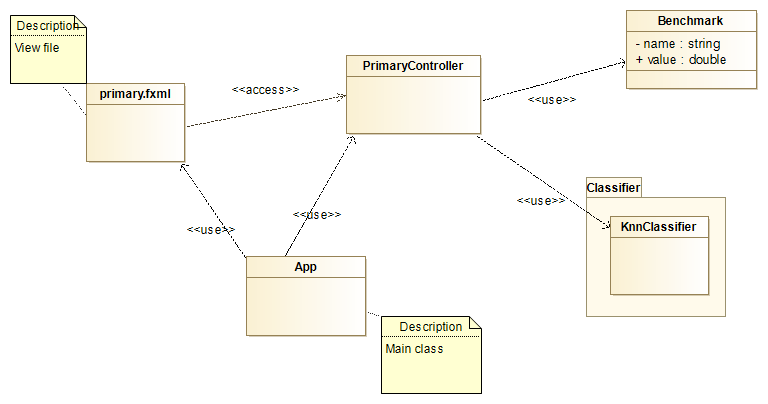
\includegraphics[width=15cm]{modul_gui.png}
    \caption{Diagram UML dla modułu GUI}
\end{figure}

\indent Zadaniem modułu DAO jest umożliwienie wczytania plików z artykułami, które zostaną poddane klasyfikacji. Implementacja tego modułu została przeprowadzona zgodnie ze wzorcem projektowym DAO, dzięki czemu dostarczony zostaje  jednolity interfejs do komunikacji między aplikacją, a źródłem danych. Poza wczytywaniem plików, w module DAO następuje także przygotowanie pliku do przetwarzania, tj. tekst zostaje poddany procesowi stematyzacji (klasa Stemm) oraz zostają usunięte najbardziej popularne słowa z języka angielskiego (klasa Stoplist), co ma na celu podniesienie jakości klasyfikacji.
\begin{figure}[H]
    \centering
    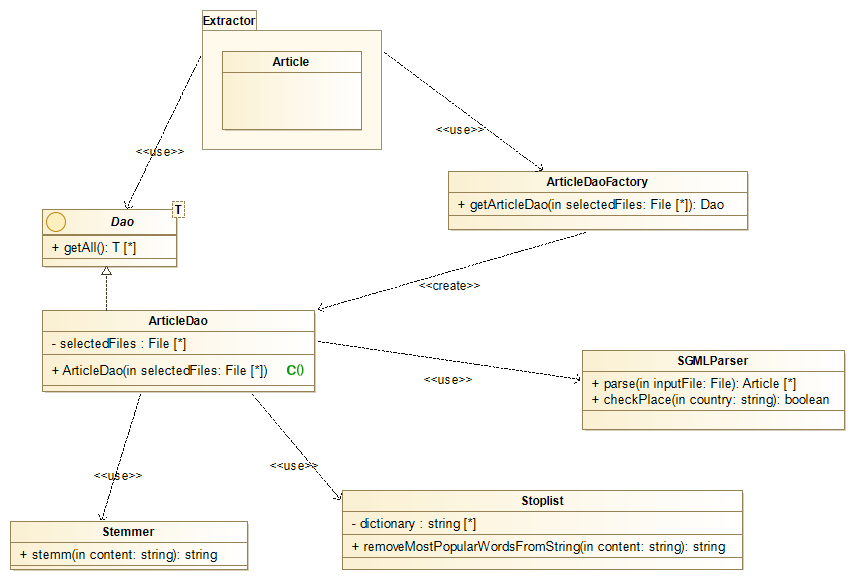
\includegraphics[width=15cm]{modul_dao.png}
    \caption{Diagram UML dla modułu DAO}
\end{figure}
\indent Moduł ekstrakcji będzie odpowiedzialny za odwzorowanie tekstu na wektor cech. Wektor cech zaimplementowany zostanie z wykorzystaniem klasy FeaturesVector. W klasie FeaturesVector znajduje się 11 pól, każde oznaczające jedną z cech, które zostały przez nas wybrane i przedstawione w sekcji 2. Dla każdej cechy stworzona została odpowiadająca klasa. Każda z klas, która reprezentuje cechę, implementuje interfejs: dla cech liczbowych jest to interfejs NumericFeature, natomiast dla cech tekstowych jest n to interfejs TextFeature.
Oba interfejsy mają metodę extract(Article article), różnica polega na zwracanej wartości. W pierwszym przypadku jest to liczba typu integer (oznaczająca obliczoną liczbę np. słów w tekście), zaś w drugim przypadku jest to lista ciągów znaków (oznaczająca wyznaczoną, znalezioną listę wyrazów, które spełniają warunki danej klasy).
\\
\begin{figure}[H]
    \centering
    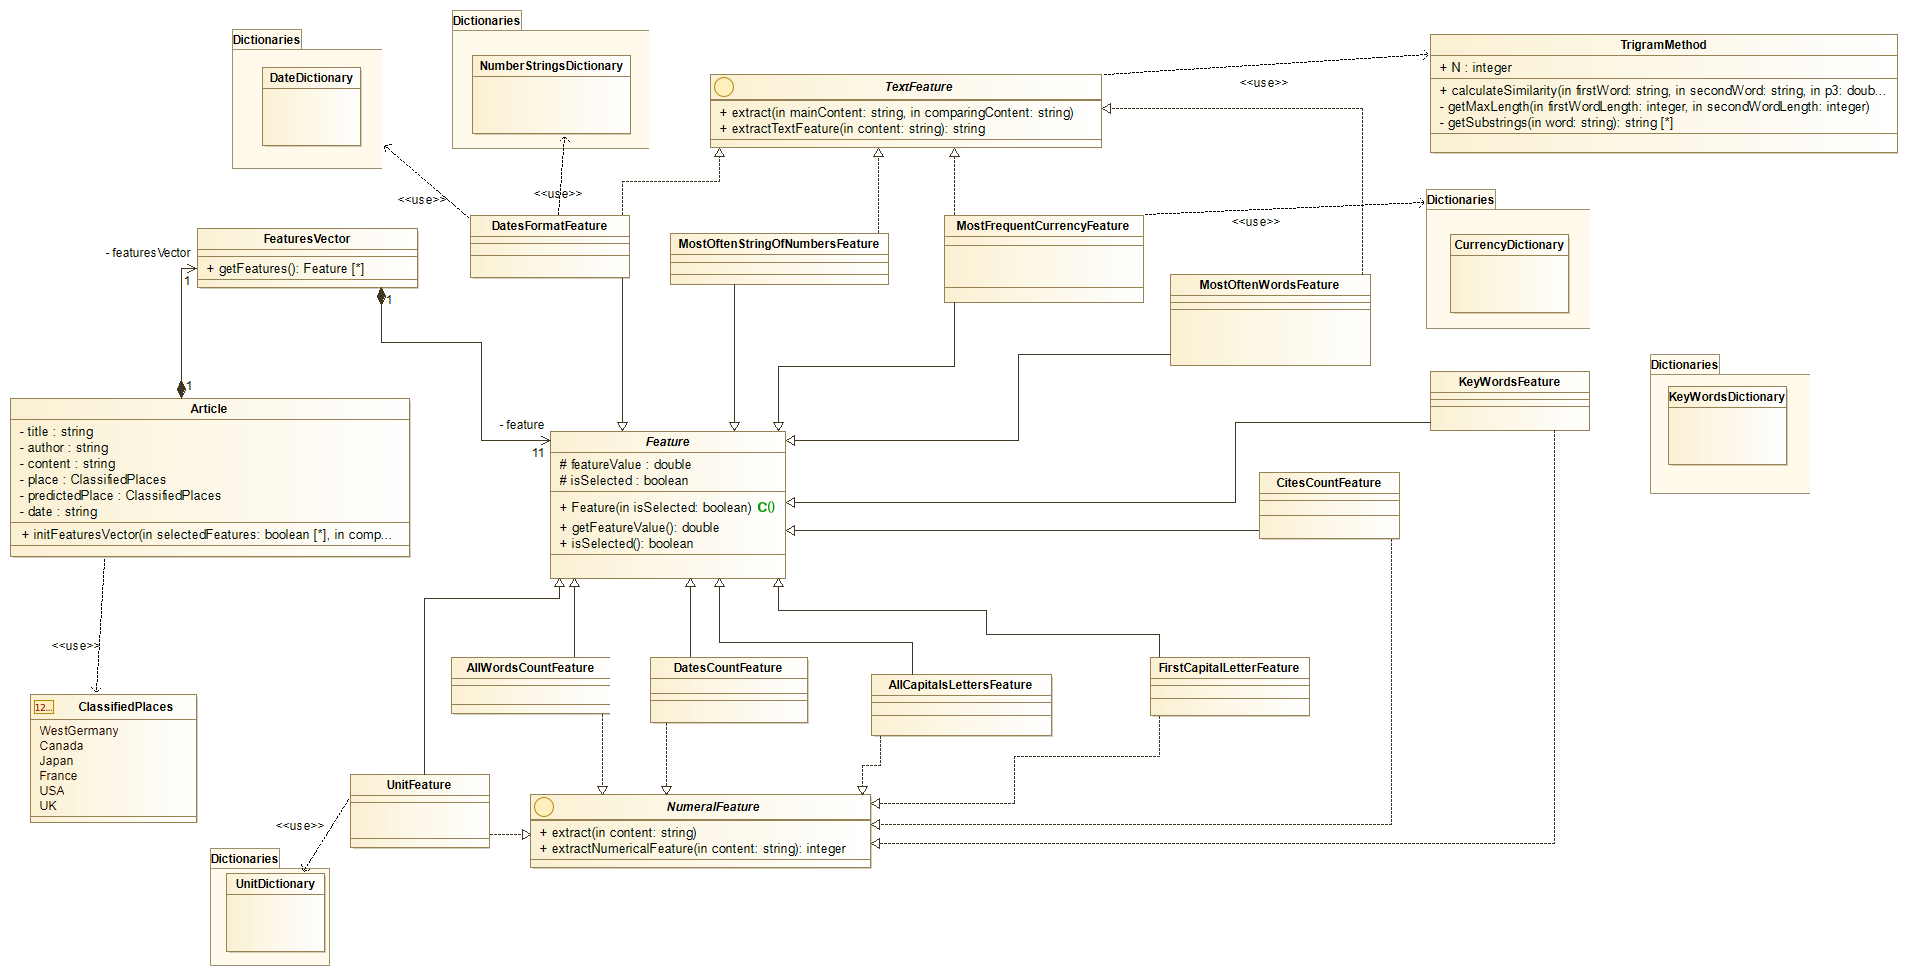
\includegraphics[width=15cm]{modul_ekstrakcji.png}
    \caption{Diagram UML dla modułu ekstrakcji}
\end{figure}


\indent Moduł klasyfikatora będzie odpowiedzialny za klasyfikację artykułów do odpowiednich etykiet places przy pomocy algorytmu kNN. Z tego względu powstanie klasa KnnClassifier, której zadaniem będzie sklasyfikowanie artykułu z wykorzystaniem jednej z trzech metryk, tj. metryki Czebyszewa, metryki ulicznej (Manhattan) lub metryki euklidesowej. W tym celu powstały cztery klasy: klasa Metric jest to klasa abstrakcyjna, natomiast klasy EuclideanMetric, ChebyshevMetric oraz ManhattanMetric są klasami dziedziczącymi. Poza metryką, niezbędne do klasyfikacji są paramtery: liczba najbliższych sąsiadów (kNeighbours) oraz stosunek liczby artykułów w części treningowej do części testowej. Do wykorzystania klasy KnnClassifier niezbędny jest moduł ekstrakcji, ponieważ klasa KnnClassifier wykorzystuje klasę Artykuł oraz kategorie ClassifiedPlaces znajdujące się w typie enumerate. \\
\begin{figure}[H]
    \centering
    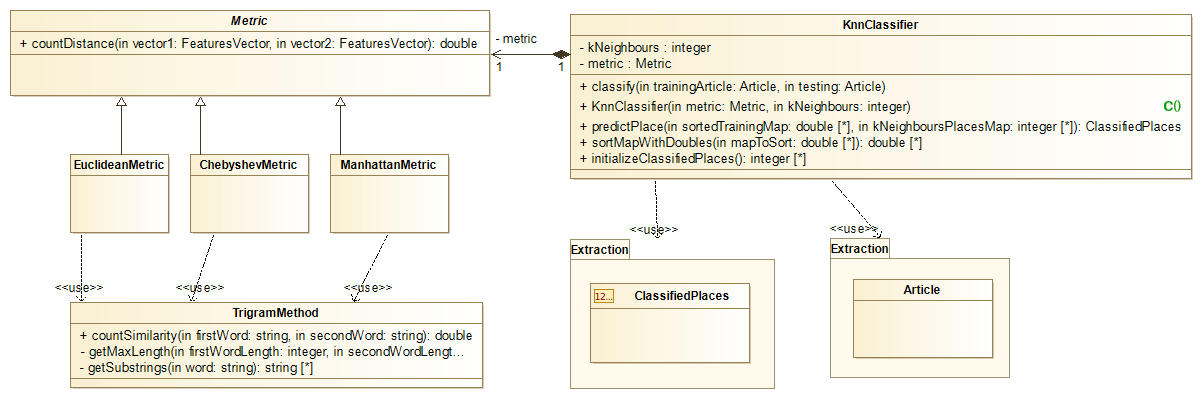
\includegraphics[width=15cm]{modul_klasyfikatora.png}
    \caption{Diagram UML dla modułu klasyfikatora}
\end{figure}

\subsection{Prezentacja wyników, interfejs użytkownika} 
Aplikacja została wykonana w technologii Java w wersji 11\cite{java_11} (najnowsza wersja LTS) przy wykorzystaniu Apache Maven w wersji 3.6.3\cite{maven}. Do stworzenia interfejsu graficznego posłużyliśmy biblioteką JavaFX w wersji 13\cite{javafx}. W celu uruchomienia aplikacji należy po zainstalowaniu Maven na własnym kpmputerze, z poziomu wiersza poleceń znajdując się w folderze głównym projektu wykonać polecenie: mvn install, a następnie z wiersza poleceń z poziomu modułu GUI wykonać polecenie: mvn clean javafx:run. Aplikacje można także uruchomić z poziomu IDE. Po uruchomieniu aplikacji ukaże nam się interfejs użytkownika, w którym możemy wybrać jak ma zostać podzielony zbiór (w jakich proporcjach na część treningową i testową), wczytać pliki, w których znajdują się teksty do analizy, podać licbę $k$ najbliższych sąsiadów dla klasyfiaktora $k$-NN, wybrać metrykę oraz zbiór cech wykorzystywanych w procesie klasyfikacji oraz wykonać klasyfikację. W efekcie ukażą nam się następujące informacje: liczba wczytanych plików, liczba artykułów podlegających klasyfikacji oraz rezultaty 4 miar podobieństwa - Accuracy, Precision, Recall i F1, a także wykres słupkowy pokazujący liczbę artykułów w każdej klasie oraz liczbę artykułów przyporządkowanej do danej klasy.
\\
\begin{figure}[H]
    \centering
    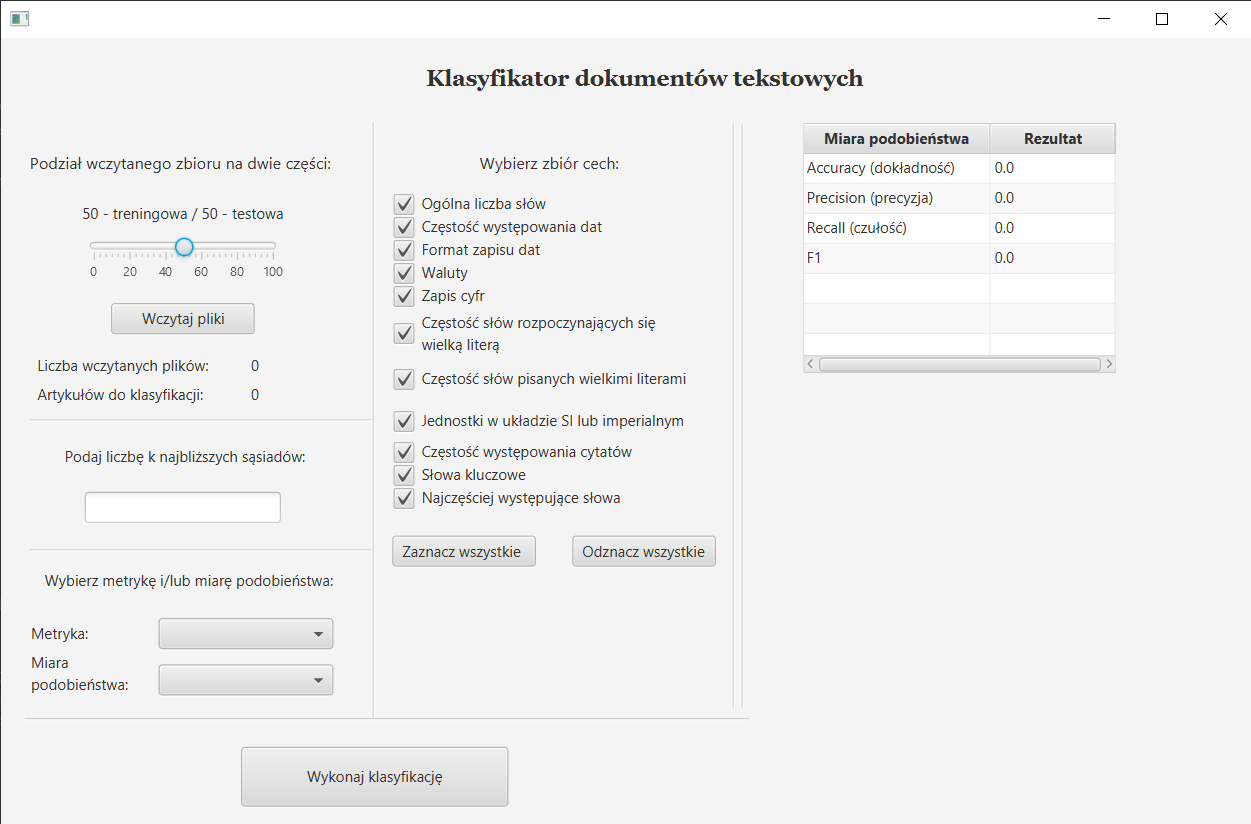
\includegraphics[width=15cm]{gui_ksr.PNG}
    \caption{Interfejs użytkownika dla aplikacji.}
\end{figure}

\section{Wyniki klasyfikacji dla różnych parametrów wejściowych}
Kolejnym krokiem było przeprowadzenie dokładnych eksperymentów dla różnych parametrów wejściowych, w celu wyciągnięcia wniosków odnośnie tego które parametry w jakim stopniu wpływają na skuteczność klasyfikacji. Eksperymenty podzieliliśmy na 4 rodzaje. Pierwszy rodzaj odnosi się do porównywania wyników klasyfikacji metody $k$-NN w zależności od różnych parametrów $k$ (przy stałych wartościach innych parametrów). Drugi rodzaj to badanie wpływu wartości podziału zbioru na wynik miar podobieństwa (Accuracy, Precision, Recall, F1). Trzecia część polegała na wyznaczeniu zależności wyników miar podobieństwa od wyboru metryki. Natomiast ostatni rodzaj eksperymentów odnosił się do badania wpływu cech na wynik klasyfikacji. Wyniki miar jakości w postaci tabel i wykresów dla wszystkich ekspermentów przedstawiono poniżej. Przeprowadzając pierwszą pulę eksperymentów dla każdego procesu klasyfikacji artykuły ze zbioru treningowego i testowego były dobierane losowo. Miało to na pewno negatywny wpływ na wyniki klasyfikacji, zatem po poprawieniu tego błędu przeprowadziliśmy drugą pulę eksperymentów.

\subsection{Porównanie wyników klasyfkacji metody $k$-NN dla różnych wartości parametru $k$}
\subsubsection{Eksperymenty dla losowego doboru artykułów do zbiorów treningowych i testowych przy każdym procesie klasyfikacji}

Podczas eksperymentów dotyczących porównania wyników klasyfikacji metody $k$-NN dla różnych wartości parametru k przyjęliśmy następujące parametry, które pozostawały niezmienne w trakcie badań:
\begin{itemize}
    \item ilość artykułów do klasyfikacji: 13531 (wszystkie)
    \item podział zbioru: 80 - treningowy/ 20 - testowy
    \item wybrana metryka: uliczna
    \item wybrane cechy: wszystkie
\end{itemize}

%tabela wygenerowana z pomoca https://www.latex-tables.com/%

% \usepackage{multirow}

\clearpage

\begin{table}
\begin{footnotesize}
\caption{Wyniki miar podobieństwa dla klasyfikacji $k$-NN w zależności od parametru $k$, gdy artykuły były przydzielane losowo do zbiorów w procesie klasyfikacji.}
\centering
\label{tabela:k}
\begin{tabular}{llllllllllll}
                                                                              & k          & 1    & 2    & 3    & 4    & 5    & 6    & 7    & 8    & 15   & 30    \\ 
\hline
\multirow{3}{*}{\begin{tabular}[c]{@{}l@{}}West-\\Germany\end{tabular}}                                                 & Precision  & 0,29 & 0,06 & 0,25 & 0,23 & 0,16 & 0,18 & 0,10 & 0,12 & 0,04 & 0,03  \\
                                                                              & Recall     & 0,32 & 0,30 & 0,67 & 0,74 & 0,53 & 0,91 & 0,60 & 0,82 & 1,00 & 1,00  \\
                                                                              & F1         & 0,30 & 0,10 & 0,36 & 0,35 & 0,24 & 0,30 & 0,16 & 0,21 & 0,08 & 0,06  \\ 
\hline
\multirow{3}{*}{Japan}                                                        & Precission & 0,73 & 0,55 & 0,80 & 0,75 & 0,74 & 0,74 & 0,77 & 0,81 & 0,83 & 0,80  \\
                                                                              & Recall     & 0,58 & 0,61 & 0,68 & 0,72 & 0,68 & 0,62 & 0,63 & 0,71 & 0,74 & 0,72  \\
                                                                              & F1         & 0,65 & 0,58 & 0,73 & 0,73 & 0,71 & 0,67 & 0,69 & 0,75 & 0,78 & 0,76  \\ 
\hline
\multirow{3}{*}{France}                                                       & Precision  & 0,69 & 0,41 & 0,51 & 0,51 & 0,57 & 0,62 & 0,65 & 0,58 & 0,59 & 0,50  \\
                                                                              & Recall     & 0,60 & 0,72 & 0,68 & 0,66 & 0,78 & 0,79 & 0,70 & 0,71 & 0,81 & 0,74  \\
                                                                              & F1         & 0,64 & 0,52 & 0,58 & 0,58 & 0,66 & 0,70 & 0,67 & 0,64 & 0,68 & 0,60  \\ 
\hline
\multirow{3}{*}{UK}                                                           & Precision  & 0,60 & 0,61 & 0,61 & 0,64 & 0,55 & 0,53 & 0,54 & 0,55 & 0,56 & 0,45  \\
                                                                              & Recall     & 0,52 & 0,43 & 0,65 & 0,60 & 0,60 & 0,61 & 0,61 & 0,66 & 0,72 & 0,69  \\
                                                                              & F1         & 0,56 & 0,51 & 0,63 & 0,62 & 0,57 & 0,57 & 0,58 & 0,60 & 0,63 & 0,55  \\ 
\hline
\multirow{3}{*}{USA}                                                          & Precision  & 0,89 & 0,84 & 0,94 & 0,94 & 0,95 & 0,96 & 0,96 & 0,96 & 0,98 & 0,98  \\
                                                                              & Recall     & 0,91 & 0,90 & 0,90 & 0,90 & 0,88 & 0,89 & 0,89 & 0,88 & 0,88 & 0,87  \\
                                                                              & F1         & 0,90 & 0,87 & 0,92 & 0,92 & 0,92 & 0,92 & 0,92 & 0,92 & 0,93 & 0,92  \\ 
\hline
\multirow{3}{*}{Canada}                                                       & Precision  & 0,33 & 0,44 & 0,28 & 0,28 & 0,18 & 0,22 & 0,21 & 0,22 & 0,09 & 0,07  \\
                                                                              & Recall     & 0,38 & 0,24 & 0,37 & 0,41 & 0,43 & 0,53 & 0,60 & 0,67 & 0,73 & 0,73  \\
                                                                              & F1         & 0,35 & 0,31 & 0,32 & 0,33 & 0,26 & 0,31 & 0,31 & 0,33 & 0,16 & 0,12  \\ 
\hline
\multirow{4}{*}{\begin{tabular}[c]{@{}l@{}}Wszystkie\\dokumenty\end{tabular}} & Accuracy   & 0,81 & 0,77 & 0,84 & 0,85 & 0,84 & 0,85 & 0,85 & 0,85 & 0,86 & 0,85  \\
                                                                              & Precsision & 0,82 & 0,76 & 0,87 & 0,88 & 0,88 & 0,90 & 0,90 & 0,91 & 0,94 & 0,94  \\
                                                                              & Recall     & 0,81 & 0,77 & 0,84 & 0,85 & 0,84 & 0,85 & 0,85 & 0,85 & 0,86 & 0,85  \\
                                                                              & F1         & 0,81 & 0,77 & 0,85 & 0,86 & 0,86 & 0,87 & 0,87 & 0,88 & 0,90 & 0,89  \\
\hline
\end{tabular}
\end{footnotesize}
\end{table}


\begin{figure}[H]
    \centering
    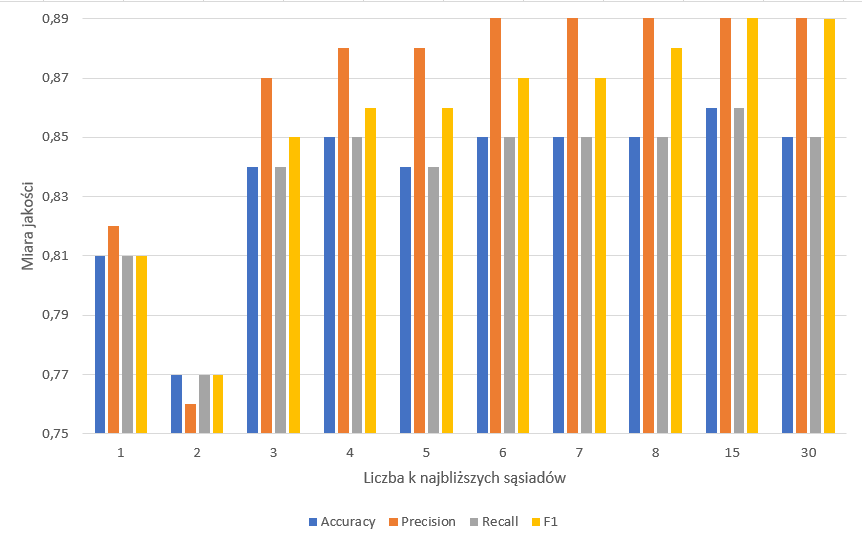
\includegraphics[width=14cm]{wykres_k.png}
    \caption{Wykres zależności wyników miar podobieństwa od liczby $k$ najbliższych sąsiadów dla klasyfikacji $k$-NN, gdy artykuły były przydzielane losowo do zbiorów w procesie klasyfi-kacji.}
    \label{wykres:k}
\end{figure}

Miara Accuracy jest najmnniejsza dla k=2, od k=3 wartości tejże miary są bardzo podobne do siebie. Warto przy tym eksperymencie zwrócić uwagę na miarę Precission, która przy bardzo dużych k (15 i 30) przyjmuje największe wartości spośród porównywanych k. Jednak, aby mieć pełny ogląd na zaistniałą sytuację należy zwrócić uwagę także na miary dla poszczególnych klas. Przy k = 15 i k = 30 miara Precision dla USA wynosi 0,98, ale już dla West-Germany odpowiednio 0,03 oraz 0,04. Co ciekawe przy tak dużych k miara Recall dla West-Germany wyniosła 1,00, co oznacza, że wartość FN (False Negative) dla tej klasy wyniosła 0. To natomiast oznacza, że nie było przypadku, że klasa element klasy West-Germany został błędnie sklasyfikowany jako element innej klasy.

\subsubsection{ Eksperymenty dla artykułów do zbiorów treningowych i testowych dobranych na stałe przy każdym procesie klasyfikacji}

Podczas eksperymentów dotyczących porównania wyników klasyfikacji metody $k$-NN dla różnych wartości parametru k przyjęliśmy następujące parametry, które pozostawały niezmienne w trakcie badań:
\begin{itemize}
    \item ilość artykułów do klasyfikacji: 13531 (wszystkie)
    \item podział zbioru: 80 - treningowy/ 20 - testowy
    \item wybrana metryka: uliczna
    \item wybrane cechy: wszystkie
\end{itemize}

\begin{table}[!htbp]
\begin{footnotesize}
\caption{Wyniki miar podobieństwa dla klasyfikacji $k$-NN w zależności od parametru $k$, gdy artykuły były przydzielane na stałe do zbiorów wprocesie klasyfikacji.}
\centering
\label{tabela:k_stale}
\begin{tabular}{llllllllllll}
                                                                              & k          & 1    & 2    & 3    & 4    & 5    & 6    & 7    & 8    & 15   & 30    \\ 
\hline
\multirow{3}{*}{\begin{tabular}[c]{@{}l@{}}West-\\Germany\end{tabular}}                                                
                                                                              & Precision  & 0,38 & 0,63 & 0,75 & 0,75 & 0,62 & 0,57 & 0,78 & 0,75 & 1,00 & 0,50  \\
                                                                              & Recall     & 0,31 & 0,19 & 0,28 & 0,17 & 0,15 & 0,15 & 0,13 & 0,06 & 0,02 & 0,02  \\
                                                                              & F1         & 0,34 & 0,29 & 0,41 & 0,27 & 0,24 & 0,24 & 0,22 & 0,10 & 0,04 & 0,04  \\ 
\hline
\multirow{3}{*}{Japan}                                                        & Precission & 0,57 & 0,59 & 0,57 & 0,65 & 0,67 & 0,70 & 0,70 & 0,70 & 0,72 & 0,69  \\
                                                                              & Recall     & 0,72 & 0,66 & 0,67 & 0,69 & 0,69 & 0,72 & 0,73 & 0,71 & 0,71 & 0,66  \\
                                                                              & F1         & 0,63 & 0,63 & 0,62 & 0,67 & 0,68 & 0,71 & 0,72 & 0,70 & 0,72 & 0,67  \\ 
\hline
\multirow{3}{*}{France}                                                       & Precision  & 0,38 & 0,73 & 0,64 & 0,64 & 0,68 & 0,64 & 0,61 & 0,65 & 0,68 & 0,64  \\
                                                                              & Recall     & 0,53 & 0,37 & 0,53 & 0,53 & 0,50 & 0,53 & 0,47 & 0,50 & 0,57 & 0,53  \\
                                                                              & F1         & 0,44 & 0,49 & 0,58 & 0,58 & 0,58 & 0,58 & 0,53 & 0,57 & 0,62 & 0,58  \\ 
\hline
\multirow{3}{*}{UK}                                                           & Precision  & 0,28 & 0,46 & 0,44 & 0,48 & 0,45 & 0,46 & 0,47 & 0,46 & 0,42 & 0,34  \\
                                                                              & Recall     & 0,32 & 0,28 & 0,36 & 0,33 & 0,34 & 0,30 & 0,31 & 0,30 & 0,26 & 0,21  \\
                                                                              & F1         & 0,30 & 0,35 & 0,40 & 0,39 & 0,38 & 0,36 & 0,37 & 0,36 & 0,32 & 0,26  \\ 
\hline
\multirow{3}{*}{USA}                                                          & Precision  & 0,91 & 0,89 & 0,90 & 0,89 & 0,89 & 0,89 & 0,89 & 0,89 & 0,88 & 0,88  \\
                                                                              & Recall     & 0,88 & 0,96 & 0,94 & 0,96 & 0,96 & 0,97 & 0,97 & 0,97 & 0,98 & 0,98  \\
                                                                              & F1         & 0,89 & 0,92 & 0,92 & 0,93 & 0,93 & 0,93 & 0,93 & 0,93 & 0,93 & 0,93  \\ 
\hline
\multirow{3}{*}{Canada}                                                       & Precision  & 0,24 & 0,39 & 0,31 & 0,40 & 0,48 & 0,55 & 0,56 & 0,61 & 0,75 & 0,75  \\
                                                                              & Recall     & 0,27 & 0,16 & 0,15 & 0,11 & 0,14 & 0,11 & 0,12 & 0,11 & 0,10 & 0,08  \\
                                                                              & F1         & 0,25 & 0,22 & 0,20 & 0,17 & 0,22 & 0,18 & 0,20 & 0,19 & 0,17 & 0,14  \\ 
\hline
\multirow{4}{*}{\begin{tabular}[c]{@{}l@{}}Wszystkie\\dokumenty\end{tabular}} & Accuracy   & 0,80 & 0,85 & 0,85 & 0,86 & 0,86 & 0,86 & 0,86 & 0,86 & 0,86 & 0,86  \\
                                                                              & Precsision & 0,81 & 0,83 & 0,83 & 0,83 & 0,83 & 0,84 & 0,84 & 0,84 & 0,85 & 0,83  \\
                                                                              & Recall     & 0,80 & 0,85 & 0,85 & 0,86 & 0,86 & 0,86 & 0,86 & 0,86 & 0,86 & 0,86  \\
                                                                              & F1         & 0,81 & 0,84 & 0,84 & 0,84 & 0,85 & 0,85 & 0,85 & 0,85 & 0,86 & 0,84  \\
\hline
\end{tabular}
\end{footnotesize}
\end{table}

\begin{figure}[H]
    \centering
    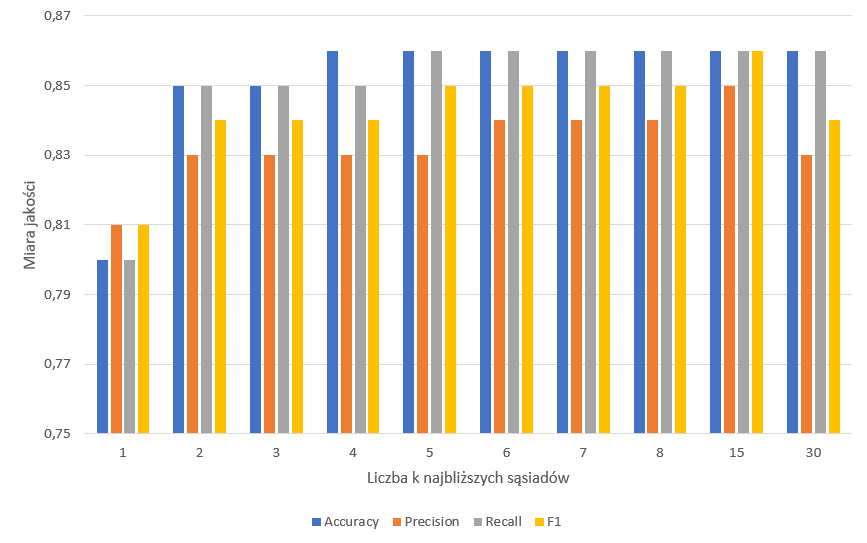
\includegraphics[width=14cm]{wykres_k_const.png}
    \caption{Wykres zależności wyników miar podobieństwa od liczby $k$ najbliższych sąsiadów dla klasyfikacji $k$-NN, gdy artykuły były przydzielane na stałe do zbiorów w procesie klasyfikacji.}
    \label{wykres:k_stale}
\end{figure}

Gdy eksperymenty przeprowadziliśmy eliminując losowe przydzielanie artykułów wyniki były bardziej "przewidywalne". Wszystkie z miar rosły, bądź pozostawały stałe podczas zwiększania liczby $k$ (poza przypadkiem zwiększenia $k$ z 15 do 30, gdzie wartości miar Precision i F1 spadły). Największt wzrost wartości miar nastąpił przy zwiększeniu $k$ z 1 do 2. Warto zwrócić także uwagę, że w tym wypadku dla coraz to większych $k$ wartość Recall zmniejszała się dla klas posiadających małą liczbę artykułów (West-Germany, Canada). Przy przydzielaniu artykułów losowo wartość ta generalnie zwiększała się (choć nie za każdym razem z uwagi właśnie na losowość), a wartość miary Precision przyjmowała bardzo małe wartościach.


\subsection{Porównanie wyników klasyfkacji metody $k$-NN w zależności od wyboru metryki}

\subsubsection{Eksperymenty dla losowego doboru artykułów do zbiorów treningowych i testowych przy każdym procesie klasyfikacji}

Podczas eksperymentów dotyczących porównania wyników klasyfikacji metody $k$-NN dla różnych metryk przyjęliśmy następujące parametry, które pozostawały niezmienne w trakcie badań:
\begin{itemize}
    \item ilość artykułów do klasyfikacji: 13531 (wszystkie)
    \item podział zbioru: 75 - treningowy/ 25 - testowy
    \item $k$ najbliższych sąsiadów: 7
    \item wybrane cechy: wszystkie
\end{itemize}

% \usepackage{multirow}

\clearpage
\begin{table}
\caption{Wyniki miar podobieństwa dla klasyfikacji $k$-NN w zależności od wybranej metryki dla wszystkich cech, gdy artykuły były przydzielane losowo do zbiorów w procesie klasyfikacji.}
\centering
\label{tabela:metryka_wszystkie}
\begin{tabular}{lllll}
                                                                              & metryka    & Czebyszewa & Uliczna & Euklidesowa  \\ 
\hline
\multirow{3}{*}{\begin{tabular}[c]{@{}l@{}}West-\\Germany\end{tabular}}       & Precision  & NaN        & 0,61    & 0,47         \\
                                                                              & Recall     & 0,00       & 0,22    & 0,19         \\
                                                                              & F1         & NaN        & 0,32    & 0,27         \\ 
\hline
\multirow{3}{*}{Japan}                                                        & Precission & NaN        & 0,60    & 0,71         \\
                                                                              & Recall     & 0,00       & 0,90    & 0,88         \\
                                                                              & F1         & NaN        & 0,72    & 0,79         \\ 
\hline
\multirow{3}{*}{France}                                                       & Precision  & NaN        & 0,76    & 0,70         \\
                                                                              & Recall     & 0,00       & 0,46    & 0,51         \\
                                                                              & F1         & NaN        & 0,57    & 0,59         \\ 
\hline
\multirow{3}{*}{UK}                                                           & Precision  & NaN        & 0,68    & 0,68         \\
                                                                              & Recall     & 0,00       & 0,51    & 0,53         \\
                                                                              & F1         & NaN        & 0,58    & 0,59         \\ 
\hline
\multirow{3}{*}{USA}                                                          & Precision  & 0,80       & 0,89    & 0,89         \\
                                                                              & Recall     & 1,00       & 0,96    & 0,97         \\
                                                                              & F1         & 0,89       & 0,92    & 0,93         \\ 
\hline
\multirow{3}{*}{Canada}                                                       & Precision  & NaN        & 0,67    & 0,65         \\
                                                                              & Recall     & 0,00       & 0,16    & 0,15         \\
                                                                              & F1         & NaN        & 0,26    & 0,24         \\ 
\hline
\multirow{4}{*}{\begin{tabular}[c]{@{}l@{}}Wszystkie\\dokumenty\end{tabular}} & Accuracy   & 0,80       & 0,85    & 0,86         \\
                                                                              & Precsision & 0,65       & 0,84    & 0,84         \\
                                                                              & Recall     & 0,81       & 0,85    & 0,86         \\
                                                                              & F1         & 0,72       & 0,85    & 0,85         \\
\hline
\end{tabular}
\end{table}

\begin{figure}[H]
    \centering
    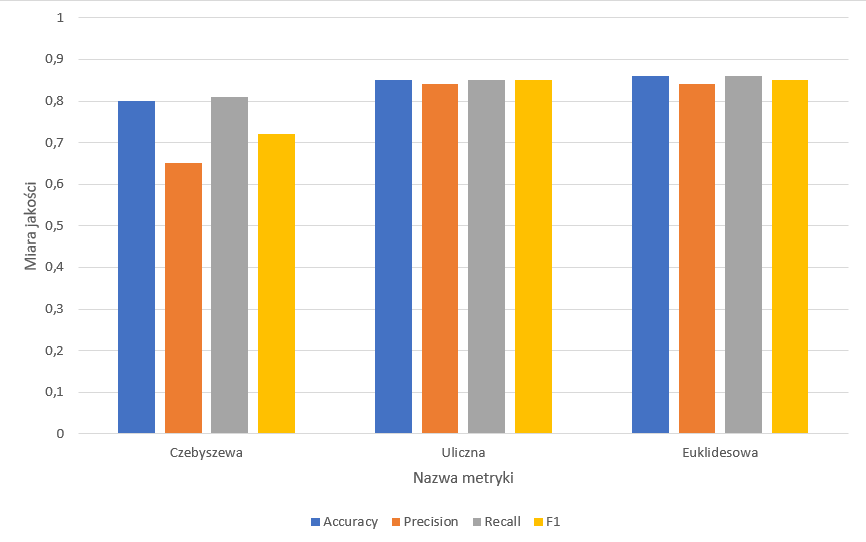
\includegraphics[width=14cm]{wykres_metryki1.png}
    \caption{Wykres zależności wyników miar podobieństwa od wybranej metryki dla wzystkich cech, gdy artykuły były przydzielane losowo do zbiorów w procesie klasyfikacji.}
        \label{wykres:metryka_wszystkie}
\end{figure}

W powyższej tabeli oraz na wykresie można zauważyć, że zdecydowanie najniższe wyniki miar podobieństwa ma metryka Czebyszewa. Również dla metryki Czebyszewa dla wszystkich krajów poza USA w mierze Precision i F1 występuje NaN, co oznacza dzielenie przez 0, co z kolei oznacza, że do tych klas nie został przydzielony żaden artykuł. Przy obliczaniu ostatecznego wyniku miary liczonego z średniej ważonej wartość NaN traktowaliśmy jako 0. Z powodu tak częstego występowania wartości NaN zdecydowaliśmy się na powtórzenie eksperymentu, tym razem stosując tylko cechy liczbowe.
Zatem, dla drugiego eksperymentu w tej sekcji przyjęliśmy następujące parametry:
\begin{itemize}
    \item ilość artykułów do klasyfikacji: 13531 (wszystkie)
    \item podział zbioru: 75 - treningowy/ 25 - testowy
    \item $k$ najbliższych sąsiadów: 7
    \item wybrane cechy: $c_3$, $c_5$, $c_6$, $c_7$, $c_8$, $c_9$.
\end{itemize}

% \usepackage{multirow}

\clearpage
\begin{table}
\caption{Wyniki miar podobieństwa dla klasyfikacji $k$-NN w zależności od wybranej metryki dla cech liczbowych, gdy artykuły były przydzielane losowo do zbiorów w procesie klasyfikacji.}
\centering
\label{table:metryka_liczbowe}
\begin{tabular}{lllll}
                                                                              & metryka    & Czebyszewa & Uliczna & Euklidesowa  \\ 
\hline
\multirow{3}{*}{\begin{tabular}[c]{@{}l@{}}West-\\Germany\end{tabular}}       & Precision  & 0,21       & 0,28    & 0,21         \\
                                                                              & Recall     & 0,06       & 0,10    & 0,12         \\
                                                                              & F1         & 0,10       & 0,14    & 0,15         \\ 
\hline
\multirow{3}{*}{Japan}                                                        & Precission & 0,25       & 0,25    & 0,25         \\
                                                                              & Recall     & 0,19       & 0,21    & 0,15         \\
                                                                              & F1         & 0,22       & 0,22    & 0,19         \\ 
\hline
\multirow{3}{*}{France}                                                       & Precision  & 0,20       & 0,29    & 0,11         \\
                                                                              & Recall     & 0,01       & 0,03    & 0,01         \\
                                                                              & F1         & 0,03       & 0,06    & 0,03         \\ 
\hline
\multirow{3}{*}{UK}                                                           & Precision  & 0,46       & 0,43    & 0,43         \\
                                                                              & Recall     & 0,23       & 0,26    & 0,25         \\
                                                                              & F1         & 0,31       & 0,32    & 0,32         \\ 
\hline
\multirow{3}{*}{USA}                                                          & Precision  & 0,83       & 0,83    & 0,84         \\
                                                                              & Recall     & 0,97       & 0,97    & 0,97         \\
                                                                              & F1         & 0,89       & 0,90    & 0,90         \\ 
\hline
\multirow{3}{*}{Canada}                                                       & Precision  & 0,36       & 0,17    & 0,27         \\
                                                                              & Recall     & 0,02       & 0,01    & 0,02         \\
                                                                              & F1         & 0,04       & 0,02    & 0,03         \\ 
\hline
\multirow{4}{*}{\begin{tabular}[c]{@{}l@{}}Wszystkie\\dokumenty\end{tabular}} & Accuracy   & 0,79       & 0,79    & 0,80         \\
                                                                              & Precsision & 0,72       & 0,72    & 0,74         \\
                                                                              & Recall     & 0,79       & 0,79    & 0,81         \\
                                                                              & F1         & 0,76       & 0,75    & 0,77         \\
\hline
\end{tabular}
\end{table}

\begin{figure}[H]
    \centering
    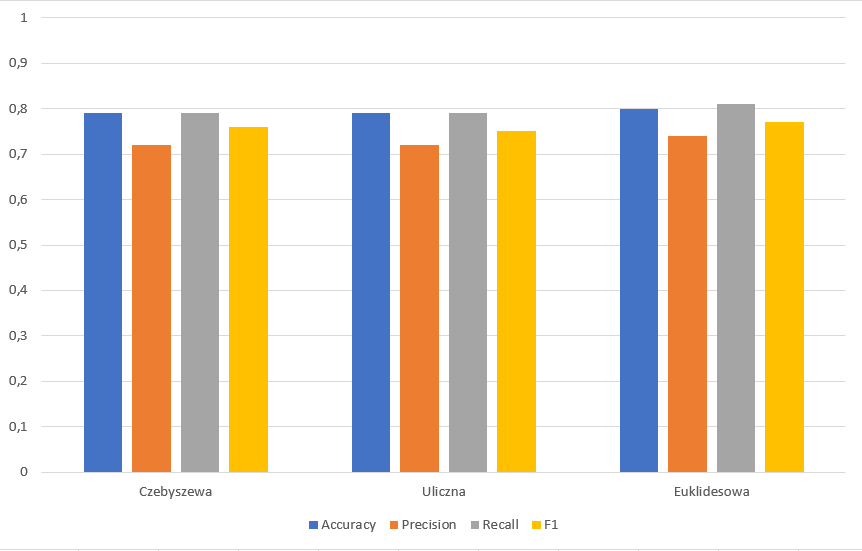
\includegraphics[width=14cm]{wykres_metryki2.png}
    \caption{Wykres zależności wyników miar podobieństwa od wybranej metryki dla cech liczbowych, gdy artykuły były przydzielane losowo do zbiorów w procesie klasyfikacji.}
        \label{wykres:metryka_liczbowe}
\end{figure}


Gdy wzięliśmy pod uwagę tylko cechy liczbowe, wyeliminowane zostały wartośći NaN przy metryce Czebyszewa. Oznacza to, że dla każdej klasy został przyporządkowany min. 1 artykuł.
\\
\subsubsection{Eksperymenty dla artykułów do zbiorów treningowych i testowych dobranych na stałe przy każdym procesie klasyfikacji}
Jako, że już wiemy, że metryka Czebyszewa nie sprawdza się dla cech tekstowych, w tej podsekcji, aby dokładniej zbadać wyniki miar w zależności od metryki, wykonamy dwa rodzaje eksperymentów - w pierwszym do badań wykorzystamy tylko cechy tekstowe, a w drugim - tylko liczbowe.\\
\indent Dla pierwszego eksperymentu w tej podsekcji przyjęliśmy następujące parametry:
\begin{itemize}
    \item ilość artykułów do klasyfikacji: 13531 (wszystkie)
    \item podział zbioru: 75 - treningowy/ 25 - testowy
    \item $k$ najbliższych sąsiadów: 7
    \item wybrane cechy: $c_1$, $c_2$, $c_4$, $c_{10}$, $c_{11}$.
\end{itemize}

\begin{table}[!htbp]
\caption{Wyniki miar podobieństwa dla klasyfikacji $k$-NN w zależności od wybranej metryki dla cech tekstowych, gdy artykuły były przydzielane na stałe do zbiorów w procesie klasyfikacji.}
\centering
\label{tabela:metryka_tesktowe_const}
\begin{tabular}{lllll}
                                                                              & metryka    & Czebyszewa & Uliczna & Euklidesowa  \\ 
\hline
\multirow{3}{*}{\begin{tabular}[c]{@{}l@{}}West-\\Germany\end{tabular}}       & Precision  & NaN        & 0,58    & 0,50         \\
                                                                              & Recall     & 0,00       & 0,09    & 0,16         \\
                                                                              & F1         & NaN        & 0,16    & 0,24         \\ 
\hline
\multirow{3}{*}{Japan}                                                        & Precission & NaN        & 0,65    & 0,68         \\
                                                                              & Recall     & 0,00       & 0,73    & 0,59         \\
                                                                              & F1         & NaN        & 0,69    & 0,63         \\ 
\hline
\multirow{3}{*}{France}                                                       & Precision  & NaN        & 0,52    & 0,55         \\
                                                                              & Recall     & 0,00       & 0,40    & 0,55         \\
                                                                              & F1         & NaN        & 0,45    & 0,55         \\ 
\hline
\multirow{3}{*}{UK}                                                           & Precision  & NaN        & 0,32    & 0,28         \\
                                                                              & Recall     & 0,00       & 0,27    & 0,28         \\
                                                                              & F1         & NaN        & 0,29    & 0,28         \\ 
\hline
\multirow{3}{*}{USA}                                                          & Precision  & 0,83       & 0,89    & 0,89         \\
                                                                              & Recall     & 1,00       & 0,96    & 0,96         \\
                                                                              & F1         & 0,90       & 0,92    & 0,92         \\ 
\hline
\multirow{3}{*}{Canada}                                                       & Precision  & NaN        & 0,76    & 0,74         \\
                                                                              & Recall     & 0,00       & 0,18    & 0,16         \\
                                                                              & F1         & NaN        & 0,29    & 0,26         \\ 
\hline
\multirow{4}{*}{\begin{tabular}[c]{@{}l@{}}Wszystkie\\dokumenty\end{tabular}} & Accuracy   & 0,83       & 0,85    & 0,85         \\
                                                                              & Precsision & 0,68       & 0,84    & 0,83         \\
                                                                              & Recall     & 0,83       & 0,85    & 0,85         \\
                                                                              & F1         & 0,75       & 0,84    & 0,84         \\
\hline
\end{tabular}
\end{table}

\begin{figure}[H]
    \centering
    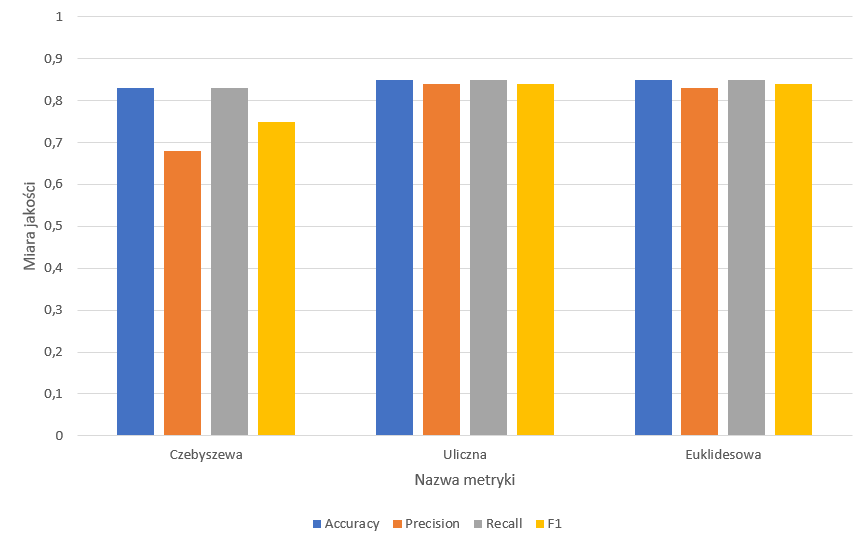
\includegraphics[width=14cm]{wykres_metryki1_const.png}
    \caption{Wykres zależności wyników miar podobieństwa od wybranej metryki dla cech tekstowych, gdy artykuły były przydzielane na stałe do zbiorów w procesie klasyfikacji.}
        \label{wykres:metryka_tekstowe_const}
\end{figure}
Potwierdziło się to, co zostało zobserwowane już, gdy artykuły były przydzielane losowo do zbiorów w procesie klasyfikacji, czyli metryka Czebyszewa nie sprawdza się dla cech tesktowych.\\
\indent Następny eksperyment polegał na zbadaniu skuteczności metryk dla cech liczbowych. Przyjęliśmy do niego następujące parametry:
\begin{itemize}
    \item ilość artykułów do klasyfikacji: 13531 (wszystkie)
    \item podział zbioru: 75 - treningowy/ 25 - testowy
    \item $k$ najbliższych sąsiadów: 7
    \item wybrane cechy: $c_3$, $c_5$, $c_6$, $c_7$, $c_8$, $c_9$.
\end{itemize}

\begin{table}[!htbp]
\caption{Wyniki miar podobieństwa dla klasyfikacji $k$-NN w zależności od wybranej metryki dla cech liczbowych, gdy artykuły były przydzielane na stałe do zbiorów w procesie klasyfikacji.}
\centering
\label{tabela:metryka_liczbowe_const}
\begin{tabular}{lllll}
                                                                              & metryka    & Czebyszewa & Uliczna & Euklidesowa  \\ 
\hline
\multirow{3}{*}{\begin{tabular}[c]{@{}l@{}}West-\\Germany\end{tabular}}       & Precision  & 0,08       & 0,10    & 0,16         \\
                                                                              & Recall     & 0,01       & 0,03    & 0,04         \\
                                                                              & F1         & 0,02       & 0,04    & 0,06         \\ 
\hline
\multirow{3}{*}{Japan}                                                        & Precission & 0,38       & 0,36    & 0,44         \\
                                                                              & Recall     & 0,09       & 0,08    & 0,12         \\
                                                                              & F1         & 0,15       & 0,14    & 0,19         \\ 
\hline
\multirow{3}{*}{France}                                                       & Precision  & 0,11       & 0,20    & 0,20         \\
                                                                              & Recall     & 0,02       & 0,02    & 0,02         \\
                                                                              & F1         & 0,04       & 0,04    & 0,04         \\ 
\hline
\multirow{3}{*}{UK}                                                           & Precision  & 0,28       & 0,25    & 0,30         \\
                                                                              & Recall     & 0,18       & 0,16    & 0,18         \\
                                                                              & F1         & 0,22       & 0,20    & 0,23         \\ 
\hline
\multirow{3}{*}{USA}                                                          & Precision  & 0,84       & 0,85    & 0,85         \\
                                                                              & Recall     & 0,97       & 0,98    & 0,98         \\
                                                                              & F1         & 0,90       & 0,91    & 0,91         \\ 
\hline
\multirow{3}{*}{Canada}                                                       & Precision  & 0,22       & 0,30    & 0,25         \\
                                                                              & Recall     & 0,03       & 0,02    & 0,02         \\
                                                                              & F1         & 0,05       & 0,03    & 0,03         \\ 
\hline
\multirow{4}{*}{\begin{tabular}[c]{@{}l@{}}Wszystkie\\dokumenty\end{tabular}} & Accuracy   & 0,82       & 0,82    & 0,82         \\
                                                                              & Precsision & 0,74       & 0,75    & 0,75         \\
                                                                              & Recall     & 0,82       & 0,82    & 0,82         \\
                                                                              & F1         & 0,78       & 0,78    & 0,78         \\
\hline
\end{tabular}
\end{table}

\begin{figure}[H]
    \centering
    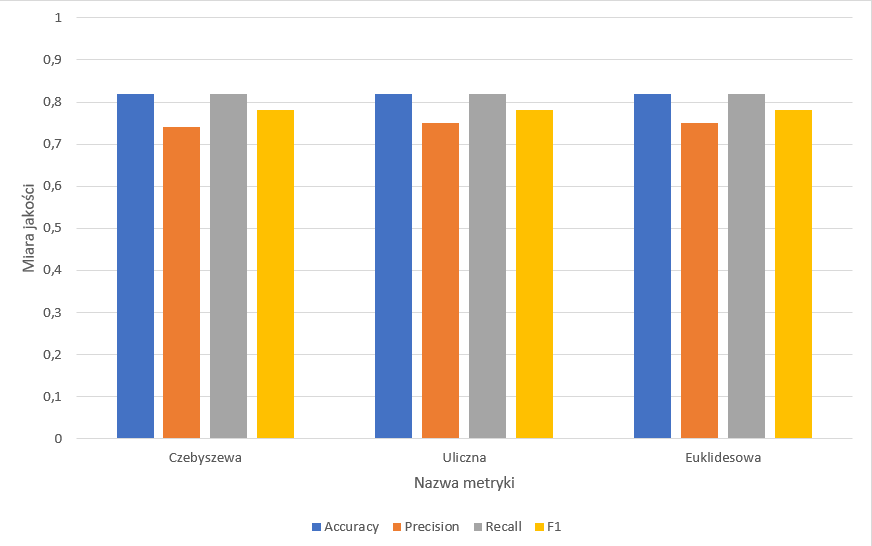
\includegraphics[width=14cm]{wykres_metryki2_const.png}
    \caption{Wykres zależności wyników miar podobieństwa od wybranej metryki dla cech liczbowych, gdy artykuły były przydzielane na stałe do zbiorów w procesie klasyfikacji.}
        \label{wykres:metryka_liczbowe_const}
\end{figure}

Jak widać w tabeli \ref{tabela:metryka_liczbowe_const} zostały wyeliminowany wartości NaN, a więc rozważając cechy liczbowe do każdej klasy przyporządkowany został co najmnniej 1 artykuł. Wyniki dla wszystkich miar są bardzo podobne (jedyną różnicą jest wartość miary Precision, która jest o 0,1 mniejsza dla metryki Czebyszewa w porównaniu z dwoma pozostałymi metrykami).

\subsection{Porównanie wyników klasyfkacji metody $k$-NN dla 5 różnych proporcji podziału zbioru artykułów}
\subsubsection{Eksperymenty dla losowego doboru artykułów do zbiorów treningowych i testowych przy każdym procesie klasyfikacji}
Podczas eksperymentów dotyczących porównania wyników klasyfikacji metody $k$-NN dla różnych proporcji podziału zbioru artykułów jako stałe parametry zostały przyjęte:
\begin{itemize}
    \item liczba artykułów do klasyfikacji: 13531 (wszystkie)
    \item liczba k-najbliższych sąsiadów: 11 
    \item wybrana metryka: uliczna
    \item wybrane cechy: wszystkie
\end{itemize}
\begin{table}[!htbp]
\caption{Wyniki klasyfikacji w zależności od proporcji podziału zbioru artykułów, gdy artykuły były przydzielane losowo do zbiorów w procesie klasyfikacji.}
\centering
\label{table:proporcja}
\begin{tabular}{cl|c|c|c|c|c|}
\cline{3-7}
\multicolumn{1}{l}{}                                 &           & \multicolumn{5}{c|}{\begin{tabular}[c]{@{}c@{}}Proporcja podziału zbioru artykułów\\  (cz. treningowa / cz. testowa)\end{tabular}} \\ \cline{3-7} 
\multicolumn{1}{l}{}                                 &           & 30/70                    & 45/55                    & 55/45                   & 70/30                   & 85/15                   \\ \hline
\multicolumn{1}{|c|}{\multirow{4}{*}{Miary jakości}} & Accuracy  & 0,84                     & 0,85                     & 0,86                    & 0,84                    & 0,86                    \\ \cline{2-7} 
\multicolumn{1}{|c|}{}                               & Precision & 0,84                     & 0,84                     & 0,85                    & 0,83                    & 0,85                    \\ \cline{2-7} 
\multicolumn{1}{|c|}{}                               & Recall    & 0,84                     & 0,85                     & 0,86                    & 0,84                    & 0,86                    \\ \cline{2-7} 
\multicolumn{1}{|c|}{}                               & F1        & 0,84                     & 0,85                     & 0,85                    & 0,84                    & 0,85                    \\ \hline
\end{tabular}
\end{table}

\clearpage
\begin{figure}[H]
    \centering
    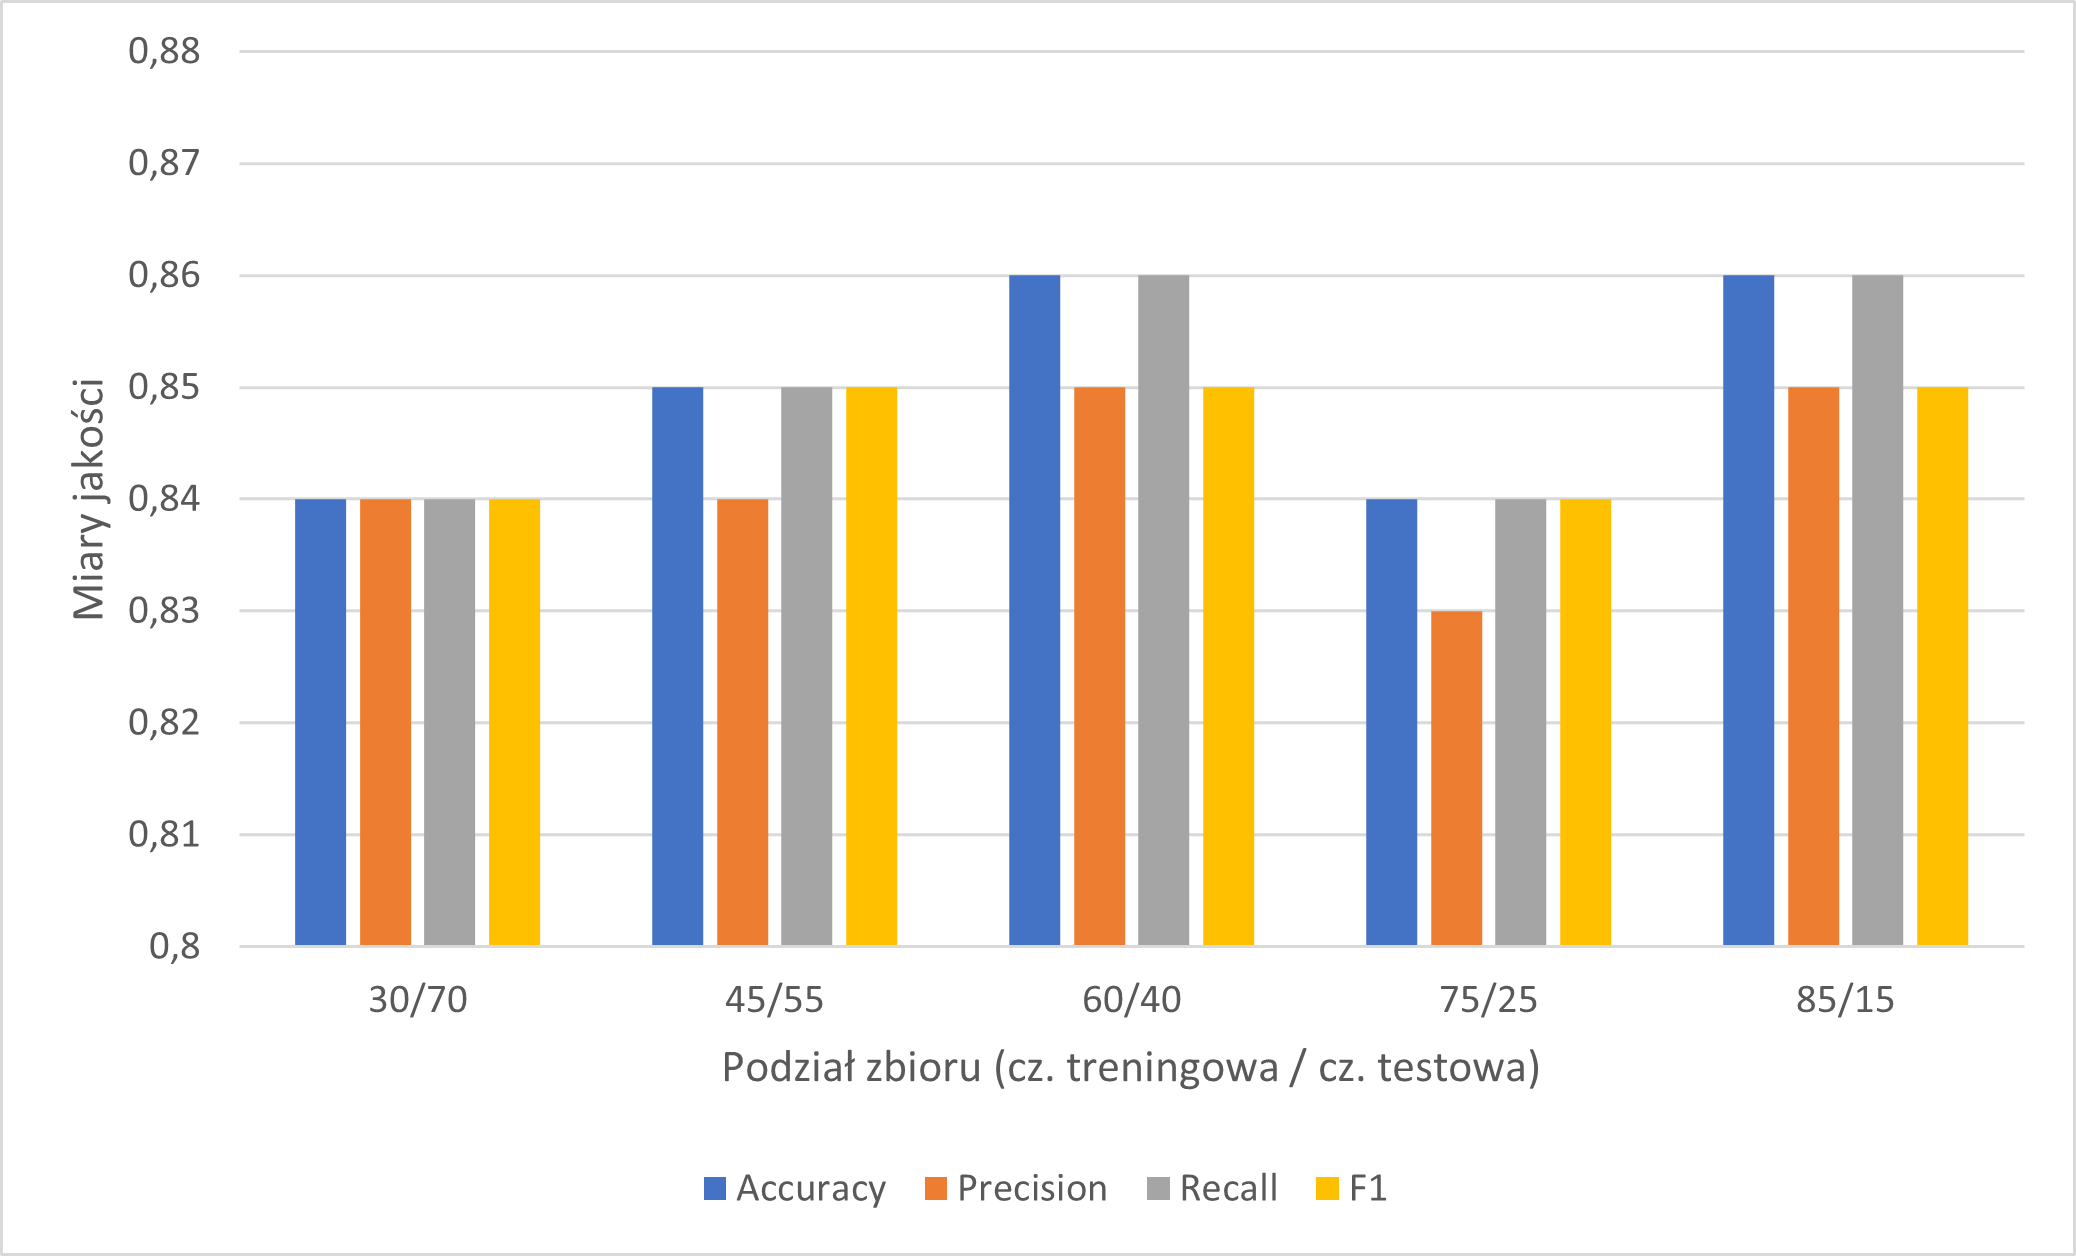
\includegraphics[width=14cm]{ranges_bar_chart.png}
    \caption{Wykres zależności wyników klasyfikacji od proporcji podziału zbioru artykułów, gdy artykuły były przydzielane losowo do zbiorów w procesie klasyfikacji.}
    \label{wykres:proporcja}
\end{figure}

\subsubsection{Eksperymenty dla artykułów do zbiorów treningowych i testowych dobranych na stałe przy każdym procesie klasyfikacji}
W kontekście badania proporcji podziału zbioru artykułow określenie "dobrane na stałe" oznacza, że przy zwiększaniu ilości artykułów w zbiorze treningowym, artykuły które były w tym zbiorze przed zmianą w nim pozostają, natomiast "dokładane" są do nich kolejne artykuły. 
\\
Podczas eksperymentów dotyczących porównania wyników klasyfikacji metody $k$-NN dla różnych proporcji podziału zbioru artykułów jako stałe parametry zostały przyjęte:
\begin{itemize}
    \item liczba artykułów do klasyfikacji: 13531 (wszystkie)
    \item liczba k-najbliższych sąsiadów: 11 
    \item wybrana metryka: uliczna
    \item wybrane cechy: wszystkie
\end{itemize}
\begin{table}[!htbp]
\caption{Wyniki klasyfikacji w zależności od proporcji podziału zbioru artykułów, gdy artykuły były przydzielane na stałe w procesie klasyfikacji.}
\centering
\label{table:proporcja_stale}
\begin{tabular}{cl|c|c|c|c|c|}
\cline{3-7}
\multicolumn{1}{l}{}                                 &           & \multicolumn{5}{c|}{\begin{tabular}[c]{@{}c@{}}Proporcja podziału zbioru artykułów\\  (cz. treningowa / cz. testowa)\end{tabular}} \\ \cline{3-7} 
\multicolumn{1}{l}{}                                 &           & 30/70                    & 45/55                    & 55/45                   & 70/30                   & 85/15                   \\ \hline
\multicolumn{1}{|c|}{\multirow{4}{*}{Miary jakości}} & Accuracy  & 0,84                     & 0,84                     & 0,84                    & 0,85                    & 0,88                    \\ \cline{2-7} 
\multicolumn{1}{|c|}{}                               & Precision & 0,81                     & 0,81                     & 0,82                    & 0,82                    & 0,85                    \\ \cline{2-7} 
\multicolumn{1}{|c|}{}                               & Recall    & 0,84                     & 0,84                     & 0,84                    & 0,85                    & 0,88                    \\ \cline{2-7}
\multicolumn{1}{|c|}{}                               & F1        & 0,82                     & 0,82                    & 0,83                    & 0,83                    & 0,86                    \\ \hline
\end{tabular}
\end{table}

\begin{figure}[H]
    \centering
    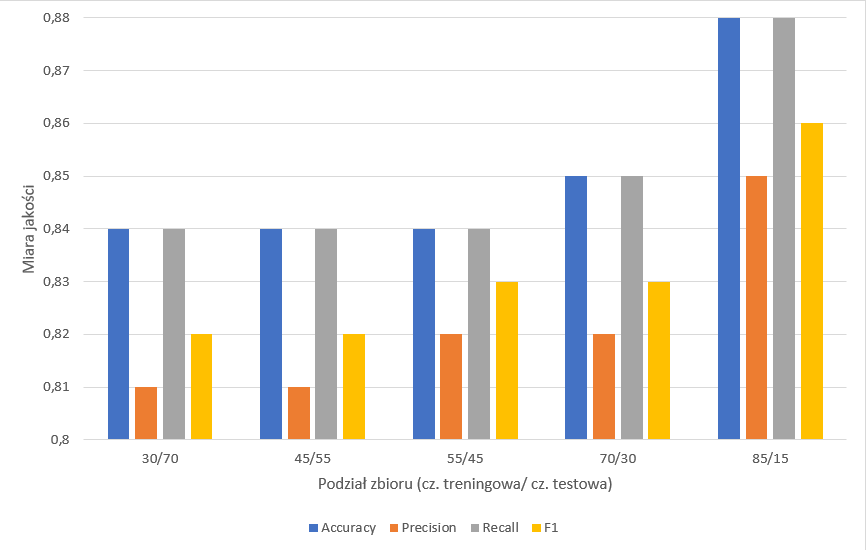
\includegraphics[width=14cm]{ranges_const_bar_chart.png}
    \caption{Wykres zależności wyników klasyfikacji w zależności od proporcji podziału zbioru artykułów, gdy artykuły były przydzielane na stałe do zbiorów w procesie klasyfikacji.}
    \label{wykres:proporcja_stale}
\end{figure}


Gdy artykuły nie były przydzielane do zbiorów losowo, wyniki miar podobieństwa były bardziej przewidywalne i sensowne. Im większa część zbioru była częścią testową tym wyniki były dokładniejsze (bądź równe wynikom z poprzedniego podziału pomiędzy podziałem 30/70, a 45/55).

\subsection{Porównanie wyników klasyfkacji metody $k$-NN dla 5 różnych podzbiorów wyekstrahowanych cech}
Podczas eksperymentów dotyczących porównania wyników klasyfikacji metody $k$-NN dla 5 różnych podzbiorów cech, jako stałe parametry zostały przyjęte:
\subsubsection {Eksperymenty dla losowego doboru artykułów do zbiorówtreningowych i testowych przy każdym procesie klasyfikacji}
\begin{itemize}
    \item liczba artykułów do klasyfikacji: 13531 (wszystkie)
    \item podział zbioru: 60 - treningowy/ 40 - testowy    
    \item liczba k-najbliższych sąsiadów: 9 
    \item wybrana metryka: Euklidesowa
\end{itemize}
Wybrane podzbiory cech w dalszej części sprawozdania będą nazywane kolejnymi zestawami, tj.:
\begin{equation}
   Zestaw1 = [c_{1}, c_{2}, c_{6}, c_{7}, c_{8}, c_{10}, c_{11}]
\end{equation}
\begin{equation}
   Zestaw2 = [c_{1}, c_{5}, c_{6}, c_{7}, c_{8}, c_{9}, c_{10}]
\end{equation}
\begin{equation}
   Zestaw3 = [c_{1}, c_{3}, c_{4}, c_{5}, c_{6}, c_{7}, c_{9}]
\end{equation}
\begin{equation}
   Zestaw4 = [c_{7}, c_{8}, c_{10}]
\end{equation}
\begin{equation}
   Zestaw5 = [c_{1}, c_{2}, c_{3}, c_{4}, c_{5}, c_{6}]
\end{equation}

\begin{table}[!htbp]
\caption{Wyniki klasyfikacji w zależności od wybranego podzbioru cech, gdy artykuły były przydzielane losowo do zbiorów w procesie klasyfikacji.}
\centering
\label{table:podzbiory}
\begin{tabular}{cl|c|c|c|c|c|}
\cline{3-7}
\multicolumn{1}{l}{}                                 &           & \multicolumn{5}{c|}{Podzbiory wyekstrahowanych cech}                                                                                                          \\ \cline{3-7} 
\multicolumn{1}{l}{}                                 &           & \multicolumn{1}{l|}{Zestaw 1} & \multicolumn{1}{l|}{Zestaw 2} & \multicolumn{1}{l|}{Zestaw 3} & \multicolumn{1}{l|}{Zestaw 4} & \multicolumn{1}{l|}{Zestaw 5} \\ \hline
\multicolumn{1}{|c|}{\multirow{4}{*}{Miary jakości}} & Accuracy  & 0,84                          & 0,85                          & 0,80                          & 0,86                          & 0,82                          \\ \cline{2-7} 
\multicolumn{1}{|c|}{}                               & Precision & 0,82                          & 0,83                          & 0,75                          & 0,85                          & 0,76                          \\ \cline{2-7} 
\multicolumn{1}{|c|}{}                               & Recall    & 0,84                          & 0,85                          & 0,80                          & 0,86                          & 0,82                          \\ \cline{2-7} 
\multicolumn{1}{|c|}{}                               & F1        & 0,83                          & 0,84                          & 0,78                          & 0,85                          & 0,80                          \\ \hline
\end{tabular}
\end{table}
\begin{figure}[H]
    \centering
    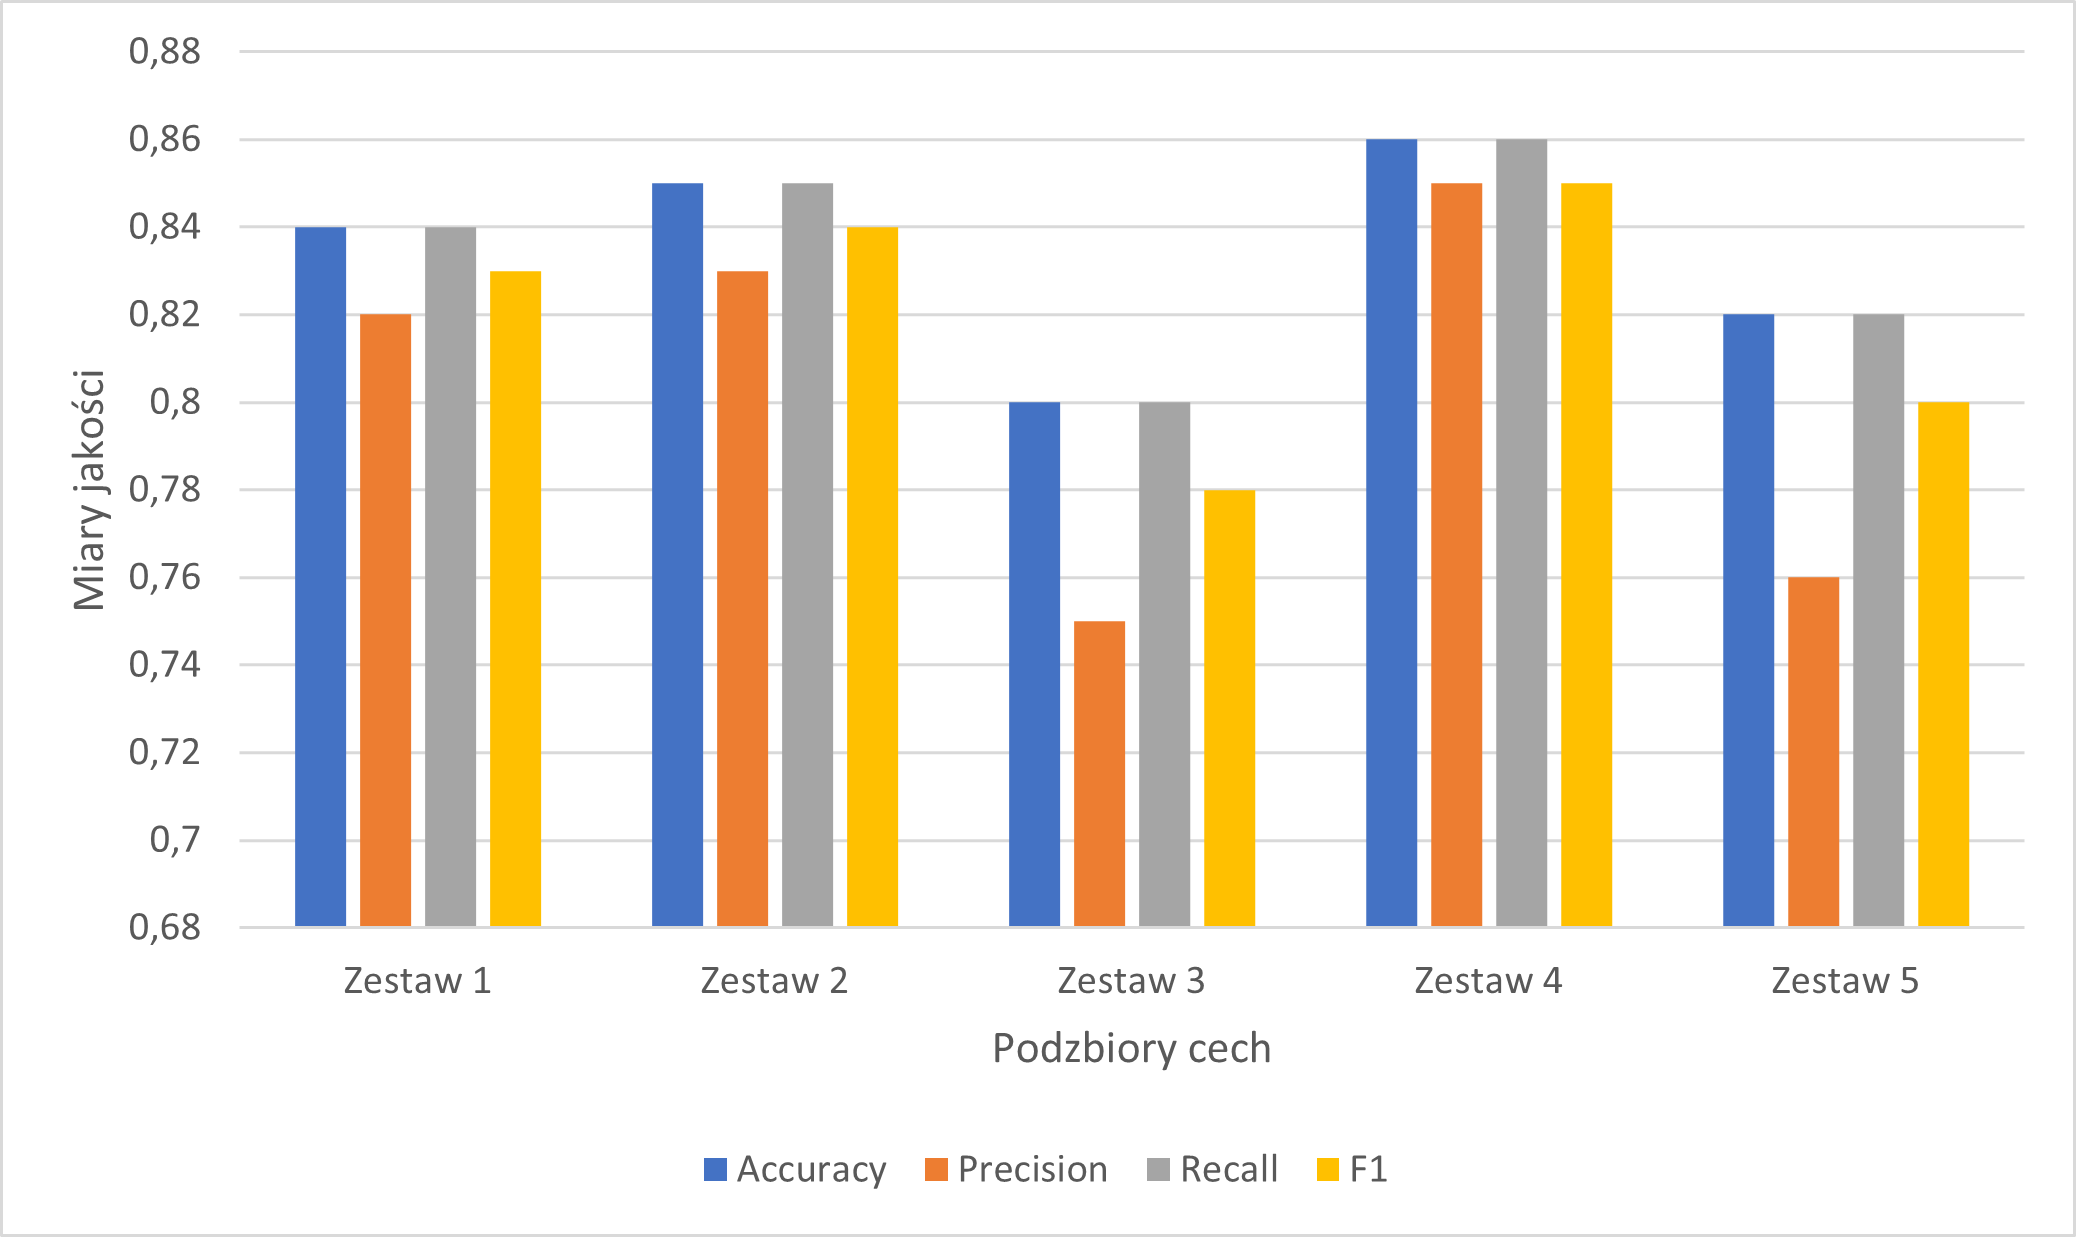
\includegraphics[width=14cm]{features_sets_bar_chart.png}
    \caption{Wykres zależności wyników klasyfikacji od podzbioru, gdy artykuły były przydzielane losowo do zbiorów w procesie klasyfikacji.}
    \label{rysunek:podzbiory}
\end{figure}
\subsubsection{Eksperymenty dla artykułów do zbiorów treningowych itestowych dobranych na stałe przy każdym procesieklasyfikacji}
\begin{itemize}
    \item liczba artykułów do klasyfikacji: 13531 (wszystkie)
    \item podział zbioru: 60 - treningowy/ 40 - testowy    
    \item liczba k-najbliższych sąsiadów: 9 
    \item wybrana metryka: Euklidesowa
\end{itemize}
Wybrane podzbiory cech w dalszej części sprawozdania będą nazywane kolejnymi zestawami, tj.:
\begin{equation}
   Zestaw1 = [c_{1}, c_{2}, c_{6}, c_{7}, c_{8}, c_{10}, c_{11}]
\end{equation}
\begin{equation}
   Zestaw2 = [c_{1}, c_{5}, c_{6}, c_{7}, c_{8}, c_{9}, c_{10}]
\end{equation}
\begin{equation}
   Zestaw3 = [c_{1}, c_{3}, c_{4}, c_{5}, c_{6}, c_{7}, c_{9}]
\end{equation}
\begin{equation}
   Zestaw4 = [c_{7}, c_{8}, c_{10}]
\end{equation}
\begin{equation}
   Zestaw5 = [c_{1}, c_{2}, c_{3}, c_{4}, c_{5}, c_{6}]
\end{equation}
\begin{table}[!htbp]
\caption{Wyniki klasyfikacji w zależności od wybranego podzbioru cech, gdy artykuły były przydzielane na stałe w procesie klasyfikacji}
\centering
\label{table:podzbiory}
\begin{tabular}{cl|c|c|c|c|c|}
\cline{3-7}
\multicolumn{1}{l}{}                                 &           & \multicolumn{5}{c|}{Podzbiory wyekstrahowanych cech}                                                                                                          \\ \cline{3-7} 
\multicolumn{1}{l}{}                                 &           & \multicolumn{1}{l|}{Zestaw 1} & \multicolumn{1}{l|}{Zestaw 2} & \multicolumn{1}{l|}{Zestaw 3} & \multicolumn{1}{l|}{Zestaw 4} & \multicolumn{1}{l|}{Zestaw 5} \\ \hline
\multicolumn{1}{|c|}{\multirow{4}{*}{Miary jakości}} & Accuracy  & 0,84                          & 0,84                          & 0,80                          & 0,85                          & 0,81                          \\ \cline{2-7} 
\multicolumn{1}{|c|}{}                               & Precision & 0,81                          & 0,82                          & 0,74                          & 0,84                          & 0,75                          \\ \cline{2-7} 
\multicolumn{1}{|c|}{}                               & Recall    & 0,84                          & 0,84                          & 0,80                          & 0,85                          & 0,81                          \\ \cline{2-7} 
\multicolumn{1}{|c|}{}                               & F1        & 0,82                          & 0,83                          & 0,77                          & 0,85                          & 0,78                          \\ \hline
\end{tabular}
\end{table}
\begin{figure}[H]
    \centering
    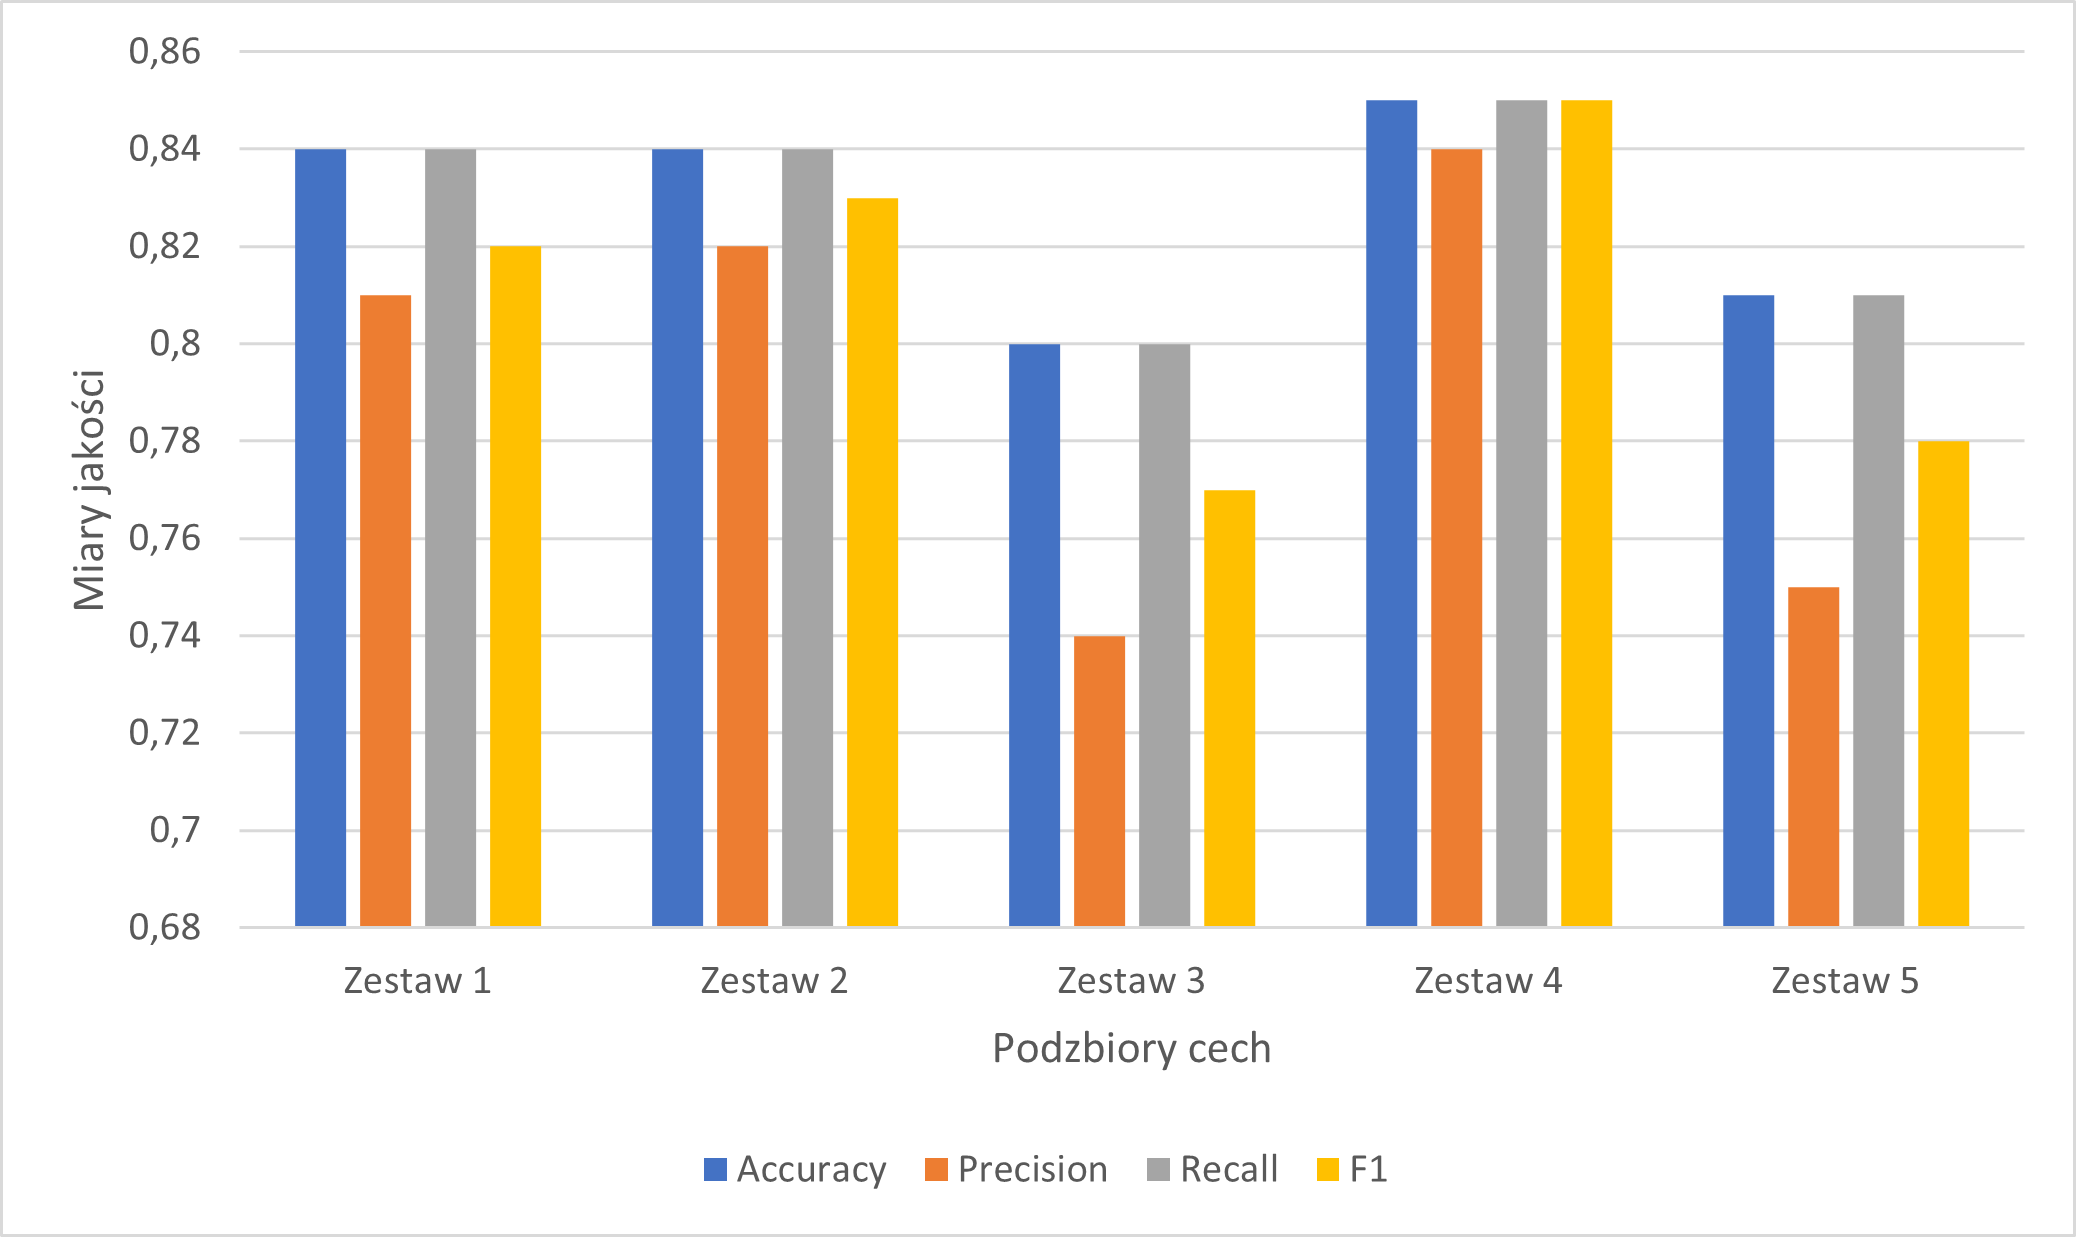
\includegraphics[width=14cm]{features_const_bar_chart.png}
    \caption{Wykres zależności wyników klasyfikacji w zależności od wybranego podzbioru cech, gdy artykuły były przydzielane na stałe do zbiorów w procesie klasyfikacji}
    \label{rysunek:podzbiory}
\end{figure}
\indent Posdumowując tą sekcję, dla metryki Ulicznej oraz Euklidesowej przy wzięciu pod uwagę wszystkich cech otrzyzmaliśmy bardzo porównywalne wyniki, które przewyższają wartości wyników dla metryki Czebyszewa. Gdy wzięliśmy pod uwagę jedynie cechy liczbowe, wszystkie metryki osiągnęły bardzo podobne wyniki. Jeśli chodzi o miarę Accuracy to metryka Euklidesowa osiągnęła o 0,1 wyższy wynik od dwóch pozostałych metryk, co pokazuje jak bliskie sobie są wszystkie trzy miary, jeśli bierzemy pod uwagę jedynie cechy liczbowe.


\clearpage
\section{Dyskusja, wnioski}
\subsection{Porównanie wyników klasyfikacji metody $k$-NN dla różnych wartości parametru $k$}

Analizując rysunek \ref{wykres:k} oraz tabelę \ref{tabela:k} (czyli wyniki dla artykułów przydzielanych losowo do zbiorów treningowych i testowych) - dla wartości $k$ mniejszych niż 3 wyniki wszystkich miar są zdecydowanie niższe porównując z wartościami $k$ większymi, bądź równymi 3. Najmniejsze wartości spośród wszystkich porównywanych wystąpiły dla $k$=2. Od $k$=3 miara Accuracy zmienia się w bardzo małym zakresie ($\pm 0,02$), możemy zatem założyć, że klasyfikator $k$-NN działa optymalnie od k=3. Ciekawie prezentuje się miara Precission, która dla większych k (15 i 30) przyjmuje zdecydowanie największą wartość (0,94). Jednak patrząc jedynie na miarę Precision dla ogółu artykułów mielibyśmy niepełne dane, które nie pozwoliłyby nam odpowiednio zinterpretować wyników. Tak duża wartość Precision występuje bowiem tylko dlatego, że dla klasy USA, która jest zdecydowanie najbardziej liczna, a co za tym idzie - ma największy wpływ na ogólny wynik, miara ta przyjmuje tak duże wartości. Patrząc na klasy odpowiadające za inne kraje wartości te są dużo mniejsze, bądź nawet bliskie zeru (West-Germany: 0,03, Canada: 0,07).\\
\indent Patrząc na rysunek \ref{wykres:k_stale} oraz tabelę \ref{tabela:k_stale}, czyli wyniki dla artykułów przydzielanych na stałe do zbiorów treningowych i testowych otrzymujemy wnioski analogiczne to tych uzyskanych powyżej, jednak z pewnymi małymi różnicami. Otóż, gdy przydzieliśmy artykuły na stałę, wyniki miar jakości rosły bądź pozostawały stałe w miarę zwiększania liczby $k$ (jedynym wyjątkiem była miara Precision oraz F1 przy zwiększeniu $k$ z 15 do 30). W tym wypadku, proporcjonalnie do zwiększania liczby $k$ zmniejszała się miara Recall dla klas, które składały się z mniejszej liczby artykułów w porówaniu z pozostałymi (West-Germany, Canada). Oznacza to, że w miarę zwiększania $k$, do klas tych było przyporządkowywane mniej artykułów. Z badania wyników klasyfikacji metody $k$-NN dla różnych wartości parametru $k$ płynie ważny wniosek - nie zawsze tylko ostateczny wynik miar podobieństwa daje nam pełny ogląd na sytuację. Należy także przeanalizować wyniki dla poszczególnych klas, aby wyciągnąć ostateczne wnioski. Ostatecznie uważamy, że najbardziej optymalną liczbą sąsiadów dla klasyfikacji metodą $k$-NN w naszym programie są liczby z przedziału $<3;7>$ 

\subsection{Porównanie wyników klasyfikacji metody $k$-NN w zależności od wyboru metryki}
W sekcji 5.2 zostały przeprowadzone 4 eksperymenty, które zostały podzielone na dwie podsekcje. Podsekcja 5.2.1 zawiera wyniki eksperymentów, gdy artykuły były przydzielane losowo do zbiorów testowych i treningowych, natomiast podsekcja 5.2.2 - wyniki, gdy artykuły były przydzielane na stałe.\\
\indent W sekcji 5.2.1 przeprowadzono dwa eksperymenty. Jeden z nich miał miejsce na wszystkich cechach (tabela \ref{tabela:metryka_wszystkie}, rysunek \ref{wykres:metryka_wszystkie}), drugi jedynie na cechach liczbowych(tabela \ref{table:metryka_liczbowe}, rysunek \ref{wykres:metryka_liczbowe}). W pierwszym eksperymencie, dla metryki Czebyszewa artykuły były przyporządkowane jedynie do klasy USA (dla pozostałych klas pojawiły się wartości NaN, co oznacza dzielenie przez zero, czyli żaden tekst nie został przyporządkowany). Stało się tak dlatego, że metryka ta jako wynik zwraca maksymaną wartość bezwzględną różnic pomiędzy kolejnymi cechami z obu wektorów. Jako, że w celu porównania dwóch cech tekstowych korzystamy z metody trigramów, a cech tekstowych jest aż pięć, zawsze zdarzy się, że porównanie którychś z tych cech zwróci wartość 1, czyli maksymalną możliwą odległość pomiędzy dwoma słowami. W niemal każdym przypadku wartość ta będzie również wartością maksymalną biorąc pod uwagę także cechy liczbowe (ponieważ cechy zostały znormalizowane, co opisano w sekcji 1). Z tego powodu przy pomocy metryki Czebyszewa, biorąc pod uwagę cechy tekstowe wszystkie teksty klasyfikowane są do jednej klasy. Dlatego metryka Czebyszewa w formie w jakiej została zaimplementowana w naszym programie nie nadaje się do cech tekstowych. Jednak przy cechach numerycznych metryka ta daje porównywalne wyniki z metryką Uliczną i Euklidesową. Metryką, która w obu eksperymentach osiągnęła najlepsze wyniki klasyfikacji była metryka Euklidesowa, która jednak bardzo nieznacznie wyprzedziła metrykę Uliczną (jeśli chodzi o miarę Accuracy było to zaledwie o 0,01 więcej).\\
\indent Eksperymenty z sekcji 5.2.2(rysunek \ref{wykres:metryka_tekstowe_const}, rysunek \ref{wykres:metryka_liczbowe_const} oraz tabele \ref{tabela:metryka_tesktowe_const} i \ref{tabela:metryka_liczbowe_const}) potwierdziły wniosek, że metryka Czebyszewa nie nadaje się do badania cech tekstowych. Dla cech tekstowych wyniki niemalże takie same (różnica była jedynie w mierze Precision i wynosiła 0,01 na korzyść metryki Ulicznej) osiągnęły metryki Uliczna i Euklidesowa. Z tego powodu uważamy, że metryki te są tak samo efektywne przy badaniu cech tekstowych. Dla cech numerycznych potwierdziły się wnioski przedstawione powyżej - wszystkie metryki osiągają niemalże identyczne wyniki miar podobieństwa. W tym wypadku jedyną różnicą jest miara Precision, która dla metryki Czebyszewa uzyskuje wartość o 0,01 mniejszą niż dla pozostałych metryk. Uważamy jednak, że dla cech numerycznych wszystkie te 3 miary mogą być używane zamiennie. Podsumowując - uważamy, że metryka Uliczna, jak i Euklidesowa jest tak samo dobrym wyborem dla klasyfikacji zbioru artykułów biorąc pod uwagę wszystkie cechy, bądź cechy tylko tekstowe. Natomiast jeśli weźmiemy pod uwagę tylko cechy liczbowe - wtedy wszytskie 3 metryki mogą być używany zamiennie.

\subsection{Porównanie wyników klasyfikacji metody $k$-NN w zależności od wybranej proporcji podziału zbioru artykułów}
W sekcji 5.3 przeprowadzone zostały dwa eksperymenty mające na celu sprawdzenie jakości klasyfikacji metodą k-NN w zależności od dobranej proporcji podziału na zbioru artykułów na część treningową i testową. W tym celu została policzona każda z miar jakości dla wszystkich dokumentów (a nie dla poszczególnych krajów, jak to miało miejsce w poprzednich sekcjach). Sekcja 5.3.1 zawiera wyniki dla losowego przydziału artykułów do zbiorów treningowych i testowych przy każdym procesie klasyfikacji, natomiast sekcja 5.3.2 - wyniki dla przydziału artykułów na stałe przy każdym procesie klasyfikacji.\\
\indent Dla sekcji 5.3.1: analizując wyniki, które zostały zawarte w (tabela \ref{tabela:proporcja}, rysunek \ref{wykres:metryka_wszystkie}) pierwszą rzeczą na którą należy zwrócić uwagę to fakt, iż wyniki dla wszystkich proporcji podziału są bardzo podobne i mieszczą się w zakresie od 0,83 do 0,86 (z dokładnością do dwóch miejsc po przecinku). Z tego względu należy uznać, że dobór proporcji podziału zbioru ma niewielki wpływ na jakość przeprowadzanej klasyfikacji. 
Jeśli spojrzymy natomiast na niewielkie różnice pomiędzy kolejnymi proporcjami można zauważyć, że dla 3 pierwszych proporcji, z każdym kolejnym badaniem wyniki minimalnie się poprawiają. Odwrócenie tego trendu następuje dopiero w przypadku 4 proporcji (75/25), dla której otrzymane wyniki są najgorsze (miara recall na poziomie 0,83). Dla 5 proporcji wyniki znowu wzrosły do poziomu takiego, jak w przypadku 3 proporcji. 
\indent W sekcji 5.3.2 wyniki są bardziej przewidywalne i sensowne. Nie następuje w tym wypadku odwrócenie trendu (jak to miało miejsce powyżej). W miarę zwiększania ilości artykułów dla części treningowej wzrasta (bądź pozostaje stała) skuteczność klasyfikacji. Zdecydowanie największy skok możemy zaobserwować przy zmianie proporcji podziału z 70/30 do 85/15. Płynie z tego wniosek, że im więcej artykułów w części treningowej w stosunku do części testowej tym skuteczniejsza jest klasyfikacja metodą $k$-NN.

\subsection{Porównanie wyników klasyfikacji metody $k$-NN w zależności od wybranego podzbioru cech}
W sekcji 5.4 przeprowadzone zostały dwa eksperymenty mające na celu sprawdzenie jakości klasyfikacji metodą k-NN w zależności od dobranego podzbioru cech artykułów. W tym celu również została policzona każda z miar jakości dla 5 różnych podzbiorów cech.  Analizując wyniki dla losowych danych, które zostały zawarte w \ref{wykres:podzbiory} oraz tabelę \ref{tabela:podzbiory} widzimy, że wyniki miar jakości są bardziej zróżnicowane, niż w przypadku eksperymentów w ramach sekcji 5.3. Najlepsze wyniki zostały otrzymane dla miary accuracy oraz recall (identyczne), natomiast najgorsze w przypadku miary precision. Pondato, możemy zauważyć większe rozbieżności pomiędzy miarą precision, a pozostałymi miarami jakości (od 0.01 w przypadku zestawu 4 do nawet 0.06 w przypadku zestawu 5). Jeśli chodzi o dobór cech, to najlepsze wyniki zostały otrzymane w przypadku zestawu 2 i zestawu 4. Wyniki dla stałego podziału artykułów na zbiory treningowy oraz testowy są bardzo podobe (minimalnie mniejsze) do tych, które zostały otrzymane dla losowych zbiorów. Różnice występujące w ramach drugiego eksperymentu wynoszą maksymalnie 0,01, więc to czy zbiory są losowe nie wpływa znacząco na jakość klasyfikacji.
Aby wykryć, które cechy mają najlepszy wpływ na klasyfikację, należy wyznaczyć część wspólną z obu zestawów o najlepszych wynikach: 
\begin{equation}
    ZestawNL = Zestaw2  \cap  Zestaw4
\end{equation}
\begin{equation}
    ZestawNL = [c_{1}, c_{5}, c_{6}, c_{7}, c_{8}, c_{9}, c_{10}] \cap [c_{7}, c_{8}, c_{10}]
\end{equation}
\begin{equation}
    ZestawNL = [c_{7}, c_{8}, c_{10}]
\end{equation}
	\indent gdzie ZestawNL oznacza wektor cech, które najbardziej pozytywnie wpływają na klasyfikację \\
\\ Z kolei do wyznaczenia cech, które w negatywny sposób wpływają na klasyfikację należy skorzystać z poniższego wzoru:
\begin{equation}
ZestawNG = Zestaw3  \cap  Zestaw5
\end{equation}
\begin{equation}
ZestawNG = [c_{1}, c_{3}, c_{4}, c_{5}, c_{6}, c_{7}, c_{9}] \cap [c_{1}, c_{2}, c_{3}, c_{4}, c_{5}, c_{6}]
\end{equation}
\begin{equation}
ZestawNG = [c_{1}, c_{3}, c_{4}, c_{5}, c_{6}]
\end{equation} 
	\indent gdzie ZestawNG oznacza wektor cech, które najmniej pozytywnie wpływają na klasyfikację \\ 
\\ Wobec tego, można uznać, że najlepszy wpływ na klasyfikację mają cechy: 
\begin{itemize}
    \item częstość słów pisanych wielkymi literami
    \item układ SI / imperialny
    \item słowa kluczowe
\end{itemize}
Z koleji cechy o najmniejszym pozytywnym wpływie na klasyfikację prezentują się następująco:
\begin{itemize}
    \item zapis cyfr
    \item częstość występowania dat
    \item format zapisu dat
    \item ogólna liczba słów
    \item format zapisu dat
    \item częstość słów rozpoczynających się wielką literą
\end{itemize}


\section*{Załączniki}
\begin{enumerate}
   \item Załącznik nr 1 - Zbiór słowników wykorzystywanych przy ekstrakcji cech.
\end{enumerate}

\begin{thebibliography}{0}
\bibitem{tadeusiewicz90} R. Tadeusiewicz: Rozpoznawanie obrazów, PWN, Warszawa, 1991.  
\bibitem{coca_words} Corpus of Contemporary American English: Most frequent english words [przeglądany  20.03.2021], Dostępny w: https://www.english-corpora.org/
\bibitem{reuters} Repozytorium Uniwersytety Kalifornijskiego w Irvine do nauki uczenia maszynowego: Artykuły agencji Reuters[przeglądany 20.03.2021], 
Dostępny w: http://archive.ics.uci.edu/ml/machine-learning-databases/reuters21578-mld/
\bibitem{niewiadomski08} A. Niewiadomski, Methods for the Linguistic Summarization of Data: Applications of Fuzzy Sets and Their Extensions, Akademicka Oficyna Wydawnicza EXIT, Warszawa, 2008.
\bibitem{tablica_pomylek} Tablica pomyłek [przeglądany 28.03.2021], Dostępny w: https://pl.wikipedia.org/wiki/Tablica\_pomyłek
\bibitem{f1} F-score [przeglądany 28.03.2021] Dostępny w: https://en.wikipedia.org/wiki/F-score
\bibitem{wyklad} A. Niewiadomski, Materiały, przykłady i ćwiczenia do przedmiotu Komputerowe Systemy Rozpoznawania, 2020.
\bibitem{java_11} Dokumetacja Java 11 [przeglądany 11.04.2021] Dostępny w : https://docs.oracle.com/en/java/javase/11/
\bibitem{maven} Dokumentacja Maven 3.6.3 [przeglądany 11.04.2021] Dostępny w: https://maven.apache.org/docs/3.6.3/release-notes.html
\bibitem{javafx} Dokumentacja JavaFx 13 [przeglądany 11.04.2021] Dostępny w: https://openjfx.io/javadoc/13/ 
\end{thebibliography}

Literatura zawiera wyłącznie źródła recenzowane i/lub o potwierdzonej wiarygodności,
możliwe do weryfikacji i cytowane w sprawozdaniu. 

\end{document}